\commentout{
\begin{code}
  module CrashCourse where
\end{code}
}

%#####################################################################
\chapter{A Crash Course in Cryptol}
\label{cha:crash-course-cryptol}

Before we can delve into cryptography, we have to get familiar with
Cryptol.  This chapter provides an introduction to Cryptol, just to
get you started. The exposition is not meant to be comprehensive, but
rather as an overview to give you a feel of the most important tools
available.  If a particular topic appears hard to approach, feel free
to skim it over for future reference.  

A full language reference is beyond the scope of this document at this
time.
% The language features not covered in this document at this time
% include:
% \begin{itemize}
% \item feature one
% \item feature two
% \end{itemize}
% \todo[inline]{2.1: Add list here of language features not yet
%   covered.}

The full grammar for Cryptol is included
in~\autoref{cha:cryptol-grammar}.

%=====================================================================
\section{Basic data types}
\label{sec:basic-data-types}

Cryptol provides four basic data types: bits, sequences, tuples, and
records.  Words (i.e., numbers) are a special case of sequences.  Note
that, aside from bits, all other Cryptol types can be nested as deep
as you like. That is, we can have records of sequences containing
tuples that comprise of other records, etc., giving us a rich
type-system for precisely describing the shapes of data our programs
manipulate.

While Cryptol is statically typed, it uses type inference to supply
unspecified types.  That is, the user does {\em not} have to write the
types of all expressions, they will be automatically inferred by the
type-inference engine.  Of course, in certain contexts the user might
choose to supply a type explicitly.  The notation is simple: we simply
put the expression, followed by {\tt :} and the type. For instance:
\begin{Verbatim}
   12 : [8]
\end{Verbatim}
means the value {\tt 12} has type {\tt [8]}, i.e., it is an 8-bit
word. We shall see other examples of this in the following discussion.

%=====================================================================
\section{Bits: Booleans}
\label{sec:bits}
\sectionWithAnswers{Bits: Booleans}{sec:bits}

The type {\tt Bit}\indTheBitType represents a single bit of
information. There are precisely two values of this type: {\tt
  True}\indTrue and {\tt False}\indFalse. Bit values play an important
role in Cryptol, as we shall see in detail shortly. In particular, the
test expression in an {\tt if-then-else} statement must have the type
{\tt Bit}.  The logical operators {\tt \&\&}\indAnd (and), {\tt
  ||}\indOr (or), {\tt \Verb|^|}\indXOr (xor), and {\tt
  \Verb|~|}\indComplement (complement) provide the basic operators
that act on bit values.

\begin{Exercise}\label{ex:dataBit}
  Type in the following expressions at the Cryptol prompt, and observe
  the output:
\begin{Verbatim}
  True
  false
  False : Bit
  if True && False then 3 else 4
  False || True
  (True && False) ^ True
  ~False
  ~(False || True)
\end{Verbatim}
Remember that Cryptol is case sensitive, and hence {\tt false} is
different from {\tt False}.\indCaseSensitive
\end{Exercise}
\begin{Answer}\ansref{ex:dataBit}
Here is the response from Cryptol, in order:
\begin{small}
\begin{Verbatim}
  True
  [error] at <interactive>:1:1--1:8: Variable `false` was not defined.
  False
  0x4
  True
  True
  True
  False
\end{Verbatim}
\end{small}
\end{Answer}

\begin{tip}
  Cryptol provides extensive command line/tab completion; use
  up/down-arrow to see your previous commands, hit tab to complete
  identifier names, etc.
\end{tip}

%=====================================================================
\section{Words: Numbers}
\label{sec:words}
\sectionWithAnswers{Words: Numbers}{sec:words}

A word is simply a numeric value, corresponding to the usual notion of
numbers.\indTheWordType To match our observation of how cryptographers
use numbers, Cryptol only supports non-negative ($\geq 0$) integer
values (i.e., no floating point or negative numbers).\indFloatingPoint
However, numbers can be arbitrarily large: There is no predefined
maximum that we are limited to.\indArbitraryPrecision By default,
Cryptol prints numbers in base 16. You might find it useful to set the
output base to be 10 while working on the following example. To do so,
use the command:\indSettingBase
\begin{Verbatim}
  :set base=10
\end{Verbatim}
The most common values for this setting are 2 (binary), 8 (octal), 10
(decimal), and 16 (hexadecimal).  Conversely, we can \emph{write}
numbers in these bases in Cryptol programs too:
\begin{Verbatim}
  0b11111011110    // binary
  0o3736           // octal
  2014             // decimal
  0x7de            // hexadecimal
\end{Verbatim}

For printing values in arbitrary bases, Cryptol uses the notation {\tt
  0<base>digits}, where base is the base value and the digits are the
numeric value in that particular base.  E.g., the above value is equal
to \texttt{0<7>5605} and \texttt{0<20>50e}.  One cannot input a value
in a non-standard base.\footnote{Cryptol does not support the input of
  numbers in arbitrary bases---the use of non-standard bases (i.e.,
  beyond base 2, 8, 10, and 16) is vanishingly rare and thus not worth
  the trouble in complicating the Cryptol parser.}

\note{Decimal numbers pose a problem in a bit-precise language like
  Cryptol.  Numbers represented in a base that is a power of two
  unambiguausly specify the number of bits required to store each
  digit.  For example {\tt 0b101} takes three bits to store. A
  hexadecimal digit takes 4 bits to store, so {\tt 0xabc} needs 12
  bits.  On the other hand, in decimal, the number of bits is
  ambiguous.  A decimal digit could require anywhere from 1 to 4 bits
  to represent.  When given a choice, Cryptol assumes the
  \emph{smallest} number of bits required to represent a decimal
  number. This is why Cryptol often prints messages like {\tt Assuming
    a = 3}; the value emitted are the number of bits necessary to
  faithfully represent the decimal value on the corresponding line.}

\todo[inline]{2.1: Make decision about
  \href{https://www.galois.com/cryptol/ticket/217}{ticket \#217} for
  the suppression of bitwidth assumption messages.}
%% If you get tired of these messages, you can suppress them with the
%% \texttt{:set reportAssuming=off} command.  Alternatively, you can
%% help Cryptol avoid from having to assume anything by using binary,
%% octal, or hexadecimal constants exclusively.  Many cryptographic
%% algorithms use decimal for their constants, but it is important to
%% keep track of how many bits they need, so the current behavior was
%% deemed a good compromise.

\begin{Exercise}\label{ex:setBase}
  Experiment with different output bases by issuing {\tt :set
    base=10}, and other base values. Also try writing numbers directly
  in different bases at the command line, such as {\tt 0o1237}.  Feel
  free to try other bases.  What is the hexadecimal version of the
  octal number {\tt 0o7756677263570015}?  Observe that {\tt :base=}
  can be set to anything between 2 and 36. Why does Cryptol stop at
  36?
\end{Exercise}
\begin{Answer}\ansref{ex:setBase}
{\tt 0xfeedfacef00d}.
Allowing base 1 would have resulted in unreadable output, and anything
larger than 36 would have required Cryptol to use unicode for digits
(and would have limited utility). As usual {\tt a} is 10, {\tt b} is
11, \ldots z is 36. Remember that upper and lower case letters denote
the same value, so {\tt a} and {\tt A} both represent 10.
\end{Answer}

\note{We will revisit the notion of numbers in
  Section~\ref{sec:words2}, after we learn about sequences.}

%=====================================================================
\section{Tuples: Heterogeneous collections}
\label{sec:tuple}
\sectionWithAnswers{Tuples: Heterogeneous collections}{sec:tuple}

A tuple is a simple collection of arbitrary ordered values of
arbitrary types, written in parentheses.\indTheTupleType A tuple is at
least a pair; it has at least two elements\footnote{Tuples with zero
  and one element are part of the underlying mathematics of Cryptol's
  tuple theory but are not supported in its concrete syntax because
  doing so unnecessarily complicates the parser and program
  comprehension.}, and can be arbitrarily nested with other types.
Elements are comma separated.  

Two tuples are equal in the standard fashion: if they have the same
arity, their types are pairwise comparable
(see~\autoref{sec:type-classes}), and their values are pairwise
identical.  Note that their types need not be pairwise identical; for
example, consider the expression \texttt{('A', 0) == (65, 0)}.  The
type of the LHS is \texttt{{a} (fin a) => ([8], [a])} while the RHS is
\texttt{{a, b} (a >= 7, fin a, fin b) => ([a], [b])}.

\todo[inline]{2.1: Decide upon the status of
  \href{https://www.galois.com/cryptol/ticket/248}{ticket \#248} wrt
  tuple semantics.  Fundamentally, why do we not support zero and one
  element tuples?}

\begin{Exercise}\label{ex:tup:1}
Try out the following tuples:
\begin{Verbatim}
  (1, 2+4)
  (True, False, True ^ False)
  ((1, 2), False, (3-1, (4, True)))
\end{Verbatim}
\end{Exercise}
\begin{Answer}\ansref{ex:tup:1}
Here are Cryptol's responses:
\begin{Verbatim}
  (1, 6)
  (True, False, True)
  ((1, 2), False, (2, (4, True)))
\end{Verbatim}
\end{Answer}

\todo[inline]{Reflect upon these computed expressions.  What is the
  operational semantics of computation of constant-valued arithmetic
  expressions?  There seems to be differing behavior between
  object-level and type-level expressions, but also differing
  semantics at the object level in different contexts.}

\paragraph*{Projecting values from tuples} Use a {\tt .} followed by
$n$ to project the $n$-th component of a tuple.  Nested projection is
not supported at this time.

\begin{Exercise}\label{ex:tup:2}
Try out the following examples:
\begin{Verbatim}
  (1, 2+4).1
  (1, 2+4).2
  ((1, 2), False, (3-1, (4, True))).3
\end{Verbatim}
\todo[inline]{Include a more interesting nested example here once
  \href{https://www.galois.com/cryptol/ticket/220}{ticket \#220} is
  fixed. As in, extract the value True, using ".2.2.2".}  Write a
projection to extract the value {\tt False} from the expression:
\begin{Verbatim}
  ((1, 2), (2, (4, True), 6), False)
\end{Verbatim}
\end{Exercise}
\begin{Answer}\ansref{ex:tup:2}
Here are Cryptol's responses:
\begin{Verbatim}
  Cryptol> (1, 2+4).1
  1
  Cryptol> (1, 2+4).2
  6
  Cryptol> ((1, 2), False, (3-1, (4, True))).3
  (2, (4, True))
\end{Verbatim}
The required expression would be:
\begin{Verbatim}
  ((1, 2), (2, (4, True), 6), False).3
\end{Verbatim}
\end{Answer}

\begin{tip}
  While projections can come in handy, we rarely see them used in
  Cryptol programs. As we shall see later, Cryptol's powerful
  pattern-matching mechanism provides a much nicer and usable
  alternative for extracting parts of tuples and other composite data
  values.
\end{tip}

%=====================================================================
\section{Sequences: Homogeneous collections}
\label{sec:sequences}
\sectionWithAnswers{Sequences: Homogeneous collections}{sec:sequences}

While tuples contain heterogeneous data, sequences are used for
homogeneous collections of values, akin to value arrays in more
traditional languages.  A sequence contains elements of any
\emph{single} type, even sequences themselves, arbitrarily nested.  We
simply write a sequence by enclosing it within square brackets with
comma-separated elements.\indTheSequenceType

\begin{Exercise}\label{ex:seq:1}
Try out the following sequences:
\begin{Verbatim}
  [1, 2]
  [[1, 2, 3], [4, 5, 6], [7, 8, 9]]
\end{Verbatim}
Note how the latter example can be used as the representation of a
$3\times3$ matrix.
\end{Exercise}

\begin{tip}
  The most important thing to remember about a sequence is that its
  elements must be of exactly the same type.
\end{tip}

\begin{Exercise}\label{ex:seq:2}
  Type in the following expressions to Cryptol and observe the
  type-errors:
\begin{Verbatim}
  [True, [True]]
  [[1, 2, 3], [4, 5]]
\end{Verbatim}
\end{Exercise}
\begin{Answer}\ansref{ex:seq:2}
In each case we get a type-error:
\begin{Verbatim}
  Cryptol> [1, True]
  [error] at <interactive>:1:1--1:10:
    Type mismatch:
      Expected type: [?a]
      Inferred type: Bit
  Cryptol> [[1, 2, 3], [4, 5]]
  [error] at <interactive>:1:1--1:20:
    Type mismatch:
      Expected type: [3][?a]
      Inferred type: [2][?b]
\end{Verbatim}
In the first case, we are trying to put a bit ({\tt True}) and a
singleton sequence containing a bit ({\tt [True]}) in the same
sequence, which have different types. In the second case, we are
trying to put two sequences of different lengths into a sequence,
which again breaks the homogeneity requirement.
\end{Answer}

%~~~~~~~~~~~~~~~~~~~~~~~~~~~~~~~~~~~~~~~~~~~~~~~~~~~~~~~~~~~~~~~~~~~~~
\subsection{Enumerations}\indEnum
\label{sec:enumerations}

Cryptol enumerations allow us to write sequences more compactly,
instead of listing the elements individually.  An enumeration is a
means of writing a sequence by providing a (possibly infinite) range.
Cryptol enumerations are not equivalent to mainstream programming
languages' notions of enumeration types, other than both kinds of
constructs guarantee that enumeration elements are distinct.

\begin{Exercise}\label{ex:seq:3}
  Explore various ways of constructing enumerations in Cryptol, by
  using the following expressions:
\begin{Verbatim}
  [1 .. 10]       // increment with step 1
  [1, 3 .. 10]    // increment with step 2 (= 3-1)
  [10, 9 .. 1]    // decrement with step 1 (= 10-9)
  [10, 9 .. 20]   // decrement with step 1 (= 10-9)
  [10, 7 .. 1]    // decrement with step 3 (= 10-7)
  [10, 11 .. 1]   // increment with step 1
\end{Verbatim}
\end{Exercise}
\begin{Answer}\ansref{ex:seq:3}
Here are the responses from Cryptol:
\begin{Verbatim}
  [1, 2, 3, 4, 5, 6, 7, 8, 9, 10]
  [1, 3, 5, 7, 9]
  [10, 9, 8, 7, 6, 5, 4, 3, 2, 1]
  []
  [10, 7, 4, 1]
  []
\end{Verbatim}
Note how {\tt [10, 11 .. 1]} and {\tt [10, 9 .. 20]} give us empty
sequences, since the upper bound is smaller than the lower bound in
the former, and larger in the latter.
\end{Answer}

%~~~~~~~~~~~~~~~~~~~~~~~~~~~~~~~~~~~~~~~~~~~~~~~~~~~~~~~~~~~~~~~~~~~~~
\subsection{Comprehensions}\indComp
\label{sec:comprehensions}

A Cryptol comprehension is a way of programmatically computing the
elements of a new sequence, out of the elements of existing
ones.\indComp  The syntax is reminiscent of the set comprehension
notation from ordinary mathematics, generalized to cover parallel
branches (as explained in the exercises below).  Note that Cryptol
comprehensions are not generalized numeric comprehensions (like
summation, product, maximum, or minimum), though such comprehensions
can certainly be defined using Cryptol comprehensions.

\begin{Exercise}\label{ex:seq:4}
  A comprehension with a single arm is called a {\em cartesian
    comprehension}. We can have one or more components in a cartesian
  comprehension.  Experiment with the following
  expressions:\indComp\indCartesian
\begin{Verbatim}
   [ (x, y) | x <- [1 .. 3], y <- [4, 5] ]
   [ x + y  | x <- [1 .. 3], y <- [] ]
   [ (x + y, z)  | x <- [1, 2], y <- [1], z <- [3, 4] ]
\end{Verbatim}
What is the number of elements in the resulting sequence, with respect
to the sizes of components?

\note{Recall that, when you type the expressions above, you will get
  messages from Cryptol such as {\tt Assuming a = 2}.  This is Cryptol
  letting you know it has decided to use 2 bits to represent, for
  example, the value {\tt 3} in {\tt [1 .. 3]}. This information may
  not seem to matter now but it can be very helpful later
  on.}
\end{Exercise}
\begin{Answer}\ansref{ex:seq:4}
Here are the responses from Cryptol:
\begin{Verbatim}
  [(1, 4) (1, 5) (2, 4) (2, 5) (3, 4) (3, 5)]
  []
  [(2, 3) (2, 4) (3, 3) (3, 4)]
\end{Verbatim}
The size of the result will be the sizes of the components
multiplied. For instance, in the first example, the generator {\tt x
  <- [1 .. 3]} assigns 3 values to {\tt x}, and the generator {\tt y
  <- [4, 5]} assigns 2 values to {\tt y}; and hence the result has
$2\times 3 = 6$ elements.
\end{Answer}

\begin{Exercise}\label{ex:seq:5}\indParallel\indComp
  A comprehension with multiple arms is called a {\em parallel
    comprehension}.  We can have any number of parallel arms. The
  contents of each arm will be {\em zipped} to obtain the results.
  Experiment with the following expressions:
\begin{Verbatim}
   [ (x, y) | x <- [1 .. 3] | y <- [4, 5] ]
   [ x + y  | x <- [1 .. 3] | y <- [] ]
   [ (x + y, z)  | x <- [1, 2] | y <- [1] | z <- [3, 4] ]
\end{Verbatim}
What is the number of elements in the resulting sequence, with respect
to the sizes of the parallel branches?
\end{Exercise}
\begin{Answer}\ansref{ex:seq:5}
Here are the responses from Cryptol:
\begin{Verbatim}
  [(1, 4) (2, 5)]
  []
  [(2, 3)]
\end{Verbatim}
In this case, the size of the result will be the minimum of the
component sizes. For the first example, the generator {\tt x <- [1
  .. 3]} assigns 3 values to {\tt x}, and the generator {\tt y <- [4,
  5]} assigns 2 values to {\tt y}; and hence the result has $\min(2,3)
= 2$ elements.
\end{Answer}

\begin{tip}
  One can mix parallel and cartesian comprehensions, where each
  parallel arm can contain multiple cartesian
  generators, or vice-versa.\indComp\indCartesian\indParallel
\end{tip}

\begin{tip}
  While Cryptol comprehensions \emph{look} like standard mathematical
  comprehensions, one must remember that the codomain of Cryptol
  comprehensions is a sequence type of some kind, \emph{not} a set.
\end{tip}

Comprehensions may be nested.\indNestedComp In this pattern, the
element value expression of the outer nesting is a sequence
comprehension (which may refer to values generated by the outer
generator). The pattern looks like this:
\begin{minipage}{\textwidth}  %% trying to avoid splitting this across pages
\begin{Verbatim}
  [  [ <expr with x & y>  //                   \
       | y <- [1 .. 5]    // inner generator    -- outer elements
     ]                                         /
     | x <- [1 .. 5]      // outer generator
  ]
\end{Verbatim}
\end{minipage}

\begin{Exercise}\label{ex:seq:6}
  Use a nested comprehension to write an expression to produce a
  $3\times3$ matrix (as a sequence of sequences), such that the $ij$th
  entry contains the value {\tt (i, j)}.
\end{Exercise}
\begin{Answer}\ansref{ex:seq:6}
  Here is one way of writing such an expression, layed out in multiple
  lines to show the structure:
\begin{Verbatim}
  [ [ (i, j) | j <- [1 .. 3] ]
     | i <- [1 .. 3]
  ]
  produces:
  [[(1, 1), (1, 2), (1, 3)], 
   [(2, 1), (2, 2), (2, 3)],
   [(3, 1), (3, 2), (3, 3)]]
\end{Verbatim}
The outer comprehension is a comprehension (and hence is nested). In
particular the expression is:
\begin{Verbatim}
     [ (i, j) | j <- [1 .. 3] ]
\end{Verbatim}
You can enter the whole expression in Cryptol all in one line, or
recall that you can put {\tt $\backslash$} at line ends to continue to
the next line.\indLineCont If you are writing such an expression in a
program file, then you can lay it out as shown above or however most
makes sense to you.
\end{Answer}

%~~~~~~~~~~~~~~~~~~~~~~~~~~~~~~~~~~~~~~~~~~~~~~~~~~~~~~~~~~~~~~~~~~~~~
\subsection{Appending and indexing}
\label{sec:appending-indexing}

For sequences, the two basic operations are appending\indAppend ({\tt
  \#}) and selecting\indIndex elements out ({\tt @}, {\tt @@}, {\tt
  !}, and {\tt !!}).  Forward selection operator ({\tt @}), starts
counting from the beginning, while the backward selection
operator\indRIndex ({\tt !}) starts from the end.  Indexing always
starts at zero: That is {\tt xs @ 0} is the first element of {\tt xs},
while {\tt xs ! 0} is the last.  The permutation\indIndexs
versions\indRIndexs ({\tt @@} and {\tt !!}, respectively) allow us to
concisely select multiple elements: they allow us to extract elements
in any order (which makes them very useful for permuting sequences).

\todo[inline]{Cite other languages that express permutations like this?}

\begin{Exercise}\label{ex:seq:7}
Try out the following Cryptol expressions:
\begin{Verbatim}
  [] # [1, 2]
  [1, 2] # []
  [1 .. 5] # [3, 6, 8]
  [0 .. 9] @ 0
  [0 .. 9] @ 5
  [0 .. 9] @ 10
  [0 .. 9] @@ [3, 4]
  [0 .. 9] @@ []
  [0 .. 9] @@ [9, 12]
  [0 .. 9] @@ [9, 8 .. 0]
  [0 .. 9] ! 0
  [0 .. 9] ! 3
  [0 .. 9] !! [3, 6]
  [0 .. 9] !! [0 .. 9]
  [0 .. 9] ! 12
\end{Verbatim}
\end{Exercise}
\begin{Answer}\ansref{ex:seq:7}
Here are Cryptol's responses:
\begin{Verbatim}
  Cryptol> :set warnDefaulting=off
  Cryptol> [] # [1, 2]
  [1, 2]
  Cryptol> [1, 2] # []
  [1, 2]
  Cryptol> [1 .. 5] # [3, 6, 8]
  [1, 2, 3, 4, 5, 3, 6, 8]
  Cryptol> [0 .. 9] @ 0
  0
  Cryptol> [0 .. 9] @ 5
  5
  Cryptol> [0 .. 9] @ 10
  invalid sequence index: 10
  Cryptol> [0 .. 9] @@ [3, 4]
  [3, 4]
  Cryptol> [0 .. 9] @@ []
  []
  Cryptol> [0 .. 9] @@ [9, 12]
  invalid sequence index: 12
  Cryptol> [0 .. 9] @@ [9, 8 .. 0]
  [9, 8, 7, 6, 5, 4, 3, 2, 1, 0]
  Cryptol> [0 .. 9] ! 0
  9
  Cryptol> [0 .. 9] ! 3
  6
  Cryptol> [0 .. 9] !! [3, 6]
  [6, 3]
  Cryptol> [0 .. 9] !! [0 .. 9]
  [9, 8, 7, 6, 5, 4, 3, 2, 1, 0]
  Cryptol> [0 .. 9] ! 12
  invalid sequence index: 12
\end{Verbatim}
\end{Answer}

\begin{Exercise}\label{ex:seq:8}
  The permutation operators ({\tt @@} and {\tt !!}) can be defined
  using sequence comprehensions.  Write an expression that selects the
  even indexed elements out of the sequence {\tt [0 .. 10]} first
  using {\tt @@}, and then using a sequence comprehension.
\end{Exercise}
\begin{Answer}\ansref{ex:seq:8}
Using a permutation operator, we can simply write:
\begin{Verbatim}
  [0 .. 10] @@ [0, 2 .. 10]
\end{Verbatim}
Using a comprehension, we can express the same idea using:
\begin{Verbatim}
  [ [0 .. 10] @ i | i <- [0, 2 .. 10] ]
\end{Verbatim}
Strictly speaking, permutation operations are indeed redundant. 
However, they lead to more concise and easier-to-read expressions.
\end{Answer}

%~~~~~~~~~~~~~~~~~~~~~~~~~~~~~~~~~~~~~~~~~~~~~~~~~~~~~~~~~~~~~~~~~~~~~
\subsection{Finite and infinite sequences}\indFiniteSeq\indInfSeq
\label{sec:finite-infin-sequ}

So far we have only seen finite sequences.  An infinite sequence is one
that has an infinite number of elements, corresponding to
streams.\indStream  Cryptol supports infinite sequences, where the
elements are accessed {\em on-demand}.  This implies that Cryptol will
{\em not} go into an infinite loop just because you have created an
infinite sequence: it will lazily construct the sequence and make its
elements available as demanded by the program.

\begin{Exercise}\label{ex:seq:9}
Try the following infinite enumerations:
\begin{Verbatim}
  [1:[32] ... ]
  [1:[32], 3 ...]
  [1:[32] ...] @ 2000
  [1:[32], 3 ...] @@ [300, 500, 700]
  [100, 102 ...]
\end{Verbatim}
\end{Exercise}
\begin{Answer}\ansref{ex:seq:9}
  When you type in an infinite sequence, Cryptol will only print the
  first 5 elements of it and will indicate that it is an infinite value
  by putting $\ldots$ at the end\footnote{You can change this behavior
    by setting the {\tt infLength} variable, like so: {\tt Cryptol>
      :set infLength=10} will show the first 10 elements of infinite
    sequences}. Here are the responses:
\begin{Verbatim}
  [1, 2, 3, 4, 5, ...]
  [1, 3, 5, 7, 9, ...]
  2001
  [601, 1001, 1401]
  [100, 102, 104, 106, 108, ...]
\end{Verbatim}
\end{Answer}
\note{Note that we are explicitly telling Cryptol to use 32-bit words
  as the elements. The reason for doing so will become clear when we
  study arithmetic shortly.}
\begin{Exercise}\label{ex:seq:10}
  What happens if you use the reverse index operator ({\tt !}) on an
  infinite sequence? Why?
\end{Exercise}
\begin{Answer}\ansref{ex:seq:10}
Here is a simple test case:
\begin{Verbatim}
  Cryptol> ([1 ... ]:[inf][32])!3

[error] at <interactive>:1:1--1:21:
  Unsolved constraint:
    fin inf
      arising from
      use of expression (!)
      at <interactive>:1:19--1:20
\end{Verbatim}
The error message is telling us that we {\em cannot} apply the reverse
index operator ({\tt !}) on an infinite sequence (\texttt{inf}).  This
is a natural consequence of the fact that one can never reach the end
of an infinite sequence to count backwards.  It is important to
emphasize that this is a {\em type-error}, i.e., the user gets this
message at compile time; instead of Cryptol going into an infinite
loop to reach the end of an infinite sequence.
\end{Answer}

%~~~~~~~~~~~~~~~~~~~~~~~~~~~~~~~~~~~~~~~~~~~~~~~~~~~~~~~~~~~~~~~~~~~~~
\subsection{Manipulating sequences} 
\label{sec:manip-sequ}

Sequences are at the heart of Cryptol, and there are a number of
built-in functions for manipulating them in various ways.  It is
worthwhile to try the following exercises to gain basic familiarity
with the basic operations.

\begin{Exercise}\label{ex:seq:11}
Try the following expressions:\indTake\indDrop\indSplitBy\indGroup\indJoin\indTranspose
\begin{Verbatim}
  take`{3} [1 .. 12]
  drop`{3} [1 .. 12]
  split`{3} [1 .. 12]
  groupBy`{3} [1 .. 12]
  join [[1 .. 4], [5 .. 8], [9 .. 12]]
  join [[1, 2, 3], [4, 5, 6], [7, 8, 9], [10, 11, 12]]
  transpose [[1, 2, 3, 4], [5, 6, 7, 8]]
  transpose [[1, 2, 3], [4, 5, 6], [7, 8, 9]]
\end{Verbatim}
And for fun, think about what these should produce:
\begin{Verbatim}
  join [1,1]
  transpose [1,2]
\end{Verbatim}
\end{Exercise}
\begin{Answer}\ansref{ex:seq:11}
Here are Cryptol's responses:
\begin{Verbatim}
  Cryptol> take`{3} [1 .. 12]
  [1, 2, 3]
  Cryptol> drop`{3} [1 .. 12]
  [4, 5, 6, 7, 8, 9, 10, 11, 12]
  Cryptol> split`{3}[1 .. 12]
  [[1, 2, 3, 4], [5, 6, 7, 8], [9, 10, 11, 12]]
  Cryptol> groupBy`{3} [1 .. 12]
  [[1, 2, 3], [4, 5, 6], [7, 8, 9], [10, 11, 12]]
  Cryptol> join [[1 .. 4], [5 .. 8], [9 .. 12]]
  [1, 2, 3, 4, 5, 6, 7, 8, 9, 10, 11, 12]
  Cryptol> join [[1, 2, 3], [4, 5, 6], [7, 8, 9], [10, 11, 12]]
  [1, 2, 3, 4, 5, 6, 7, 8, 9, 10, 11, 12]
  Cryptol> transpose [[1, 2, 3, 4], [5, 6, 7, 8]]
  [[1, 5], [2, 6], [3, 7], [4, 8]]
  Cryptol> transpose [[1, 2, 3], [4, 5, 6], [7, 8, 9]]
  [[1, 4, 7], [2, 5, 8], [3, 6, 9]]
\end{Verbatim}
\todo[inline]{Add discussion about join[1,1] and transpose [1,2].}
\todo[inline]{Why is isn't join in the prelude?!}
\end{Answer}

\begin{Exercise}\label{ex:seq:12}
  Based on your intuitions from the previous exercise, derive laws
  between the following pairs of functions: {\tt take} and {\tt drop};
  {\tt join} and {\tt split}; {\tt join} and {\tt groupBy}; {\tt
    split} and {\tt groupBy} and {\tt transpose} and itself.  For
  instance, {\tt take} and {\tt drop} satisfy the following
  equality:\indTake\indDrop\indJoin\indSplitBy\indGroup\indTranspose
\begin{Verbatim}
   (take`{n} xs) # (drop`{n} xs) == xs
\end{Verbatim}
whenever {\tt n} is between {\tt 0} and the length of the sequence
{\tt xs}. Note that there might be multiple laws these functions
satisfy.
\end{Exercise}
\begin{Answer}\ansref{ex:seq:12}
  The following equalities are the simplest
  candidates:\indJoin\indSplitBy\indGroup\indTranspose
\begin{Verbatim}
  join (split`{parts=n} xs) == xs
  join (groupBy`{each=n} xs) == xs
  split`{parts=n} xs == groupBy`{each=m} xs
  transpose (transpose xs) == xs
\end{Verbatim}
In the first two equalities {\tt n} must be a divisor of the length of
the sequence {\tt xs}.  In the third equation, {\tt n} $\times$ {\tt m}
must equal the length of the sequence {\tt xs}.
\todo[inline]{These are theorems that should be part of the prelude!}
\end{Answer}

\begin{Exercise}\label{ex:seq:13}
What is the relationship between the append operator {\tt \#} and {\tt
  join}?\indAppend\indJoin
\end{Exercise}
\begin{Answer}\ansref{ex:seq:13}
Append ({\tt \#})\indAppend\indJoin joins two sequences of arbitrary
length, while {\tt join} appends a sequence of equal length
sequences. In particular, the equality:
\begin{Verbatim}
   join [xs0, xs1, xs2, .. xsN] = xs0 # xs1 # xs2 ... # xsN
\end{Verbatim}
holds for all equal length sequences {\tt xs0}, {\tt xs1}, $\ldots$,
{\tt xsN}.
\end{Answer}

\paragraph*{Type-directed splits} We have studied the functions {\tt
  groupBy}\indGroup and {\tt splitBy}\indSplit above.  Cryptol also
provides a function {\tt split}\indSplit that can split a sequence
into any number of equal-length segments.  A common way to use {\tt
  split} is to be explicit about the type of its result, instead of
passing arguments as we did above with {\tt splitBy} and {\tt
  groupBy}.
\begin{Verbatim}
  Cryptol> split [1..12] : [1][12][8]
  [[1, 2, 3, 4, 5, 6, 7, 8, 9, 10, 11, 12]]
  Cryptol> split [1..12] : [2][6][8]
  [[1, 2, 3, 4, 5, 6], [7, 8, 9, 10, 11, 12]]
  Cryptol> split [1..12] : [3][4][8]
  [[1, 2, 3, 4], [5, 6, 7, 8], [9, 10, 11, 12]]
\end{Verbatim}
Here is what happens if we do {\em not} give an explicit signature on
the result:\indSignature
\begin{Verbatim}
  Cryptol> split [1..12]
  <polymorphic value>
  Cryptol> :t split [1..12]
  split [1 .. 12] : {a, b, c} (a >= 4, fin a, fin c,
                              12 == b * c) => [b][c][a]
\end{Verbatim}
%% cryptol 1 said: : {a b c} (fin c,c >= 4,a*b == 12) => [a][b][c]

A complex type signature like this one first defines a set of type
variables {\tt \Verb|{a, b, c}|}, a set of constraints on those
variables {\tt \Verb|(a >= 4, fin a, fin c, 12 == b * c)|}, a {\tt =>}
and finally the shape description.  In this case, Cryptol's {\tt
  [b][c][a]} is telling us that the result will be a sequence of {\tt
  b} things, each of which is a sequence of {\tt c} things, each of
which is a word of size {\tt a}. The type constraints tell us that
{\tt a} is at least 4, because the maximum element of the sequence is 12,
and it takes at least 4 bits to represent the value 12.  The
constraints are that {\tt b * c == 12}, which means we should
completely cover the entire input, and that the lengths {\tt a} and
{\tt c} need to be finite.  As you can see, {\tt split} is a very
powerful function. The flexibility afforded by {\tt split} comes in
very handy in Cryptol.  We shall see one example of its usage later in
Section~\ref{sec:scytale}.

\begin{Exercise}\label{ex:split:0}
  With a sequence of length 12, as in the above example, there are
  precisely 6 ways of splitting it: 1--12, 2--6, 3--4, 4--3, 6--2, and
  12--1. We have seen the first three splits above. Write the
  expressions corresponding to the latter 3.\indSplit
\end{Exercise}
\begin{Answer}\ansref{ex:split:0}
Here they are:\indSplit
\begin{Verbatim}
  Cryptol> split [1..12] : [4][3][8]
  [[1, 2, 3], [4, 5, 6], [7, 8, 9], [10, 11, 12]]
  Cryptol> split [1..12] : [6][2][8]
  [[1, 2], [3, 4], [5, 6], [7, 8], [9, 10], [11, 12]]
  Cryptol> split [1..12] : [12][1][8]
  [[1], [2], [3], [4], [5], [6], [7], [8], [9], [10], [11], [12]]
\end{Verbatim}
\end{Answer}

\begin{Exercise}\label{ex:split:1}
  What happens when you type {\tt split [1 .. 12] :
    [5][2][8]}?\indSplit
\end{Exercise}
\begin{Answer}\ansref{ex:split:1}
Cryptol will issue a type error:\indSplit
\begin{Verbatim}
  Cryptol> split [1..12] : [5][2][8]
  Unsolved constraint:
    1 + (12 - 1) == 5 * 2
      arising from
      matching types
      at <interactive>:1:1--1:16
\end{Verbatim}
Cryptol is telling us that we have requested 10 elements in the final
result (5*2), but the input has 12.
\end{Answer}

\begin{Exercise}\label{ex:split:2}
  Write a {\tt split} expression to turn the sequence {\tt [1 .. 120]
    : [120][8]} into a nested sequence with type {\tt [3][4][10][8]},
  keeping the elements in the same order.\indSplit \lhint{Use nested
    comprehensions.}  \indComp
\end{Exercise}
\begin{Answer}\ansref{ex:split:2}
  We can split\indSplit 120 elements first into 3--40, splitting each
  of the the elements ({\tt level1} below) into 4--10. A nested
  comprehension fits the bill:\indComp
\begin{Verbatim}
  [ split level1 : [4][10][8]
  | level1 <- split ([1 .. 120] : [120][8]) : [3][40][8]
  ]
\end{Verbatim}
(Note again that you can enter the above in the command line all in
one line, or by putting the line continuation character {\tt
  $\backslash$} at the end of the first two lines.)\indLineCont
\end{Answer}

%~~~~~~~~~~~~~~~~~~~~~~~~~~~~~~~~~~~~~~~~~~~~~~~~~~~~~~~~~~~~~~~~~~~~~
\subsection{Shifts and rotates} 
\label{sec:shifts-rotates}

Common operations on sequences include shifting and rotating them.
Cryptol supports both versions with left/right
variants.\indShiftLeft\indShiftRight\indRotLeft\indRotRight
\begin{Exercise}\label{ex:seq:14}
Experiment with the following expressions:
\begin{Verbatim}
   [1, 2, 3, 4, 5] >> 2
   [1, 2, 3, 4, 5] >> 10
   [1, 2, 3, 4, 5] << 2
   [1, 2, 3, 4, 5] << 10
   [1, 2, 3, 4, 5] >>> 2
   [1, 2, 3, 4, 5] >>> 10
   [1, 2, 3, 4, 5] <<< 2
   [1, 2, 3, 4, 5] <<< 10
\end{Verbatim}
\noindent Notice that shifting/rotating always returns a sequence
precisely the same size as the original.
\end{Exercise}
\begin{Answer}\ansref{ex:seq:14}
Here are Cryptol's responses:
\begin{Verbatim}
  [0, 0, 1, 2, 3]
  [0, 0, 0, 0, 0]
  [3, 4, 5, 0, 0]
  [0, 0, 0, 0, 0]
  [4, 5, 1, 2, 3]
  [1, 2, 3, 4, 5]
  [3, 4, 5, 1, 2]
  [1, 2, 3, 4, 5]
\end{Verbatim}
\todo[inline]{Reflections on this exercise?}
\end{Answer}
\begin{Exercise}\label{ex:seq:15}
  Let {\tt xs} be a sequence of length $n$. What is the result of
  rotating {\tt xs} left or right by a multiple of $n$?
\end{Exercise}
\begin{Answer}\ansref{ex:seq:15}
  Rotating (left or right) by a multiple of the size of a sequence
  will leave it unchanged.
\end{Answer}

%=====================================================================
\section{Words revisited}
\label{sec:words2}
\sectionWithAnswers{Words revisited}{sec:words2}

In Section~\ref{sec:words} we have introduced numbers as a distinct
value type in Cryptol. In fact, a number in Cryptol is nothing but a
finite sequence of bits, so words are not a separate type. For
instance, the literal expression {\tt 42} is precisely the same as the
bit-sequence corresponding to {\tt [True, False, True, False, True,
  False]}.\indTheWordType

\begin{Exercise}\label{ex:words:0}
  Explain why {\tt 42} is the same as {\tt [True, False, True, False,
    True, False]}.  Is Cryptol little-endian, or
  big-endian?\indEndianness
\end{Exercise}
\begin{Answer}\ansref{ex:words:0}
  Cryptol is big-endian,\indEndianness meaning that the
  most-significant-bit comes first. In the sequence {\tt [True, False,
    True, False, True, False]}, the first element corresponds to the
  most-significant-digit, i.e., $2^5$, the next element corresponds to
  the coefficient of $2^4$, etc.  A {\tt False} bit yields a
  coefficient of $0$ and a {\tt True} bit gives $1$. Hence, we have:
$$1\times2^5 + 0\times2^4 + 1\times2^3 + 0\times2^2 + 1\times2^1 + 0\times2^0 = 32 + 0 + 8 + 0 + 2 + 0 = 42$$
\end{Answer}

\begin{Exercise}\label{ex:words:1}
  Try out the following words: \lhint{It might help to use {\tt :set
      base=2} to see the bit patterns.}\indSettingBase
\begin{Verbatim}
  12
  12 # [False]
  [False, False] # 12
  [True, False] # 12
  12 # [False, True]
  32
  12 # 32
  [True, False, True, False, True, False] == 42
\end{Verbatim}
\end{Exercise}
\begin{Answer}\ansref{ex:words:1}
  After issuing {\tt :set base=2}, here are Cryptol's
  responses:\indSettingBase
\begin{Verbatim}
  0b1100
  0b11000
  0b1100
  0b101100
  0b110001
  0b100000
  0b1100100000
  True
\end{Verbatim}
\end{Answer}

\begin{Exercise}\label{ex:words:2}
  What is the type of {\tt 0}?  Use the {\tt :t} command to find this
  out.  (Type {\tt :t 0} at the prompt.\indSettingType) Are there any
  other elements of this type? What are the elements of the type {\tt
    [2]}?
\end{Exercise}
\begin{Answer}\ansref{ex:words:2}
{\tt 0} has the type {\tt \Verb+{a} [a]+}.
Incidentally, {\tt 0} is the only value that inhabits this type. The
type {\tt [2]} is precisely inhabited by the elements {\tt 0, 1, 2,}
and {\tt 3}.
\todo[inline]{Reflect upon the fact that zero has no length component.}
\end{Answer}

\paragraph*{Defaulting and explicit types}\indDefaulting Top level
polymorphic constants in a Cryptol program are subject to
{\em defaulting}, meaning that Cryptol will use the fewest number of
bits necessary to represent them. Users can override this by giving an
explicit type signature.\indSignature

\begin{Exercise}\label{ex:words:3}
  \todo[inline]{\href{https://www.galois.com/cryptol/ticket/83}{Ticket \#83}
    must be addressed before we can include the text: ``For this
    exercise, first issue {\tt :set +t} command...''.}  Try the
  following expressions:
\begin{Verbatim}
  :t 42
  :t 42 : [9]
  :t 42 : [3]
\end{Verbatim}
Can you jam more bits in a word than is potentially possible in
Cryptol?  Compare this behavior to a typical C expression: {\tt (char)
  9999}.
\end{Exercise}
\begin{Answer}\ansref{ex:words:3}
  The number 42 needs at least 6 bits to represent; hence the last
  expression fails. Note how type-inference helps, as users can give
  type annotations only when they need to be more specific.  Unlike
  the C example, Cryptol will statically make sure that there will not
  be any overflow.
\end{Answer}

\begin{Exercise}\label{ex:words:4}
Since words are sequences, the sequence functions from
Exercise~\ref{sec:sequences}--\ref{ex:seq:11} apply to words as well. Try out
the following examples and explain the outputs you
observe:\indTake\indDrop\indSplit\indGroup
\begin{Verbatim}
  take`{3} 0xFF
  take`{3} (12:[6])
  drop`{3} (12:[6])
  split`{3} (12:[6])
  groupBy`{3} (12:[6])
\end{Verbatim}
\end{Exercise}
\noindent Recall that the notation {\tt 12:[6]} means the constant 12
with the type precisely 6-bits wide.
\begin{Answer}\ansref{ex:words:4}
  Remember that Cryptol is big-endian\indEndianness and hence {\tt
    12:[6]} is precisely {\tt [False, False, True, True, False,
    False]}.  Here are Cryptol's responses:\indTake
\begin{Verbatim}
  Cryptol> take`{3} 0xFF
  7
  Cryptol> take`{3} (12:[6])
  1
  Cryptol> drop`{3} (12:[6])
  4
  Cryptol> split`{3} (12:[6])
  [0, 3, 0]
  Cryptol> groupBy`{3} (12:[6])
  [1, 4]
\end{Verbatim}
For instance, the expression {\tt take`\{3\} (12:[6])} evaluates as follows:
\begin{Verbatim}
  take`{3} (12:[6])
    = take (3, [False, False, True, True, False, False])
    = [False, False, True]
    = 1
\end{Verbatim}
Follow similar lines of reasoning to justify the results for the
remaining expressions.
\end{Answer}
\begin{Exercise}\label{ex:words:5}
  Try Exercise~\ref{ex:words:4}, this time with the constant {\tt
    12:[12]}. Do any of the results change? Why?
\end{Exercise}
\begin{Answer}\ansref{ex:words:5}
  Because of the leading zeros in {\tt 12:[12]}, they all produce
  different results:\indTake\indDrop\indSplit\indGroup
\begin{Verbatim}
  Cryptol> take`{3} (12:[12])
  0
  Cryptol> drop`{3} (12:[12])
  12
  Cryptol> split`{3} (12:[12])
  [0, 0, 12]
  Cryptol> groupBy`{3} (12:[12])
  [0, 0, 1, 4]
\end{Verbatim}
We will show the evaluation steps for {\tt groupBy} here, and urge the
reader to do the same for {\tt splitBy}:
\begin{Verbatim}
  groupBy`{3} (12:[12])
    = groupBy`{3} [False, False, False, False, False, False, 
                   False, False, True, True, False, False]
    = [[False, False, False], [False, False, False] 
       [False, False, True], [True, False, False]]
    = [0, 0, 1, 4]
\end{Verbatim}
\end{Answer}

\paragraph*{Shifts and rotates on words} Consider what happens if we
shift a word, say {\tt 12:[6]} by one to the right:
\indShiftLeft\indShiftRight\indRotLeft\indRotRight
\begin{Verbatim}
  (12:[6]) >> 1
    = [False, False, True, True, False, False] >> 1
    = [False, False, False, True, True, False]
    = 6 
\end{Verbatim}
That is shifting-right by one effectively divides the word by 2. This
is due to Cryptol's ``big-endian'' representation of
numbers\footnote{This is a significant change from Cryptol version 1,
  which interpreted the leftmost element of a sequence as the
  lowest-ordered bit (and thus shifting right was multiplying by 2,
  and shifting left was dividing by 2). The way it is handled now
  matches the traditional
  interpretation.}.\indRotLeft\indRotRight\indShiftLeft\indShiftRight

\begin{Exercise}\label{ex:words:6}
Try the following examples of shifting/rotating words:
\begin{Verbatim}
  (12:[8]) >> 2
  (12:[8]) << 2
\end{Verbatim}
\end{Exercise}
\begin{Answer}\ansref{ex:words:6}
Here are Cryptol's responses:
\begin{Verbatim}
  3
  48
\end{Verbatim}
\todo[inline]{Reflect upon these responses.}
\end{Answer}

\todo[inline]{2.0: This is \textbf{NOT} architecture endianness; we
  need a better discussion here.  Dylan will do some code-diving on
  Cryptol version 1.}

\paragraph*{Little-endian vs Big-endian} The discussion of endianness
comes up often in computer science, with no clear
winner.\indEndianness Since Cryptol allows indexing from the beginning
or the end of a (finite) sequence, you can access the 0th
(least-significant) bit of a sequence $k$ with $k$!0, the 1st bit with
$k$!1, and so on.\indIndex

%=====================================================================
\section{Characters and strings}
\label{sec:charstring}

Strictly speaking Cryptol does {\em not} have characters and strings
as a separate type. However, Cryptol does allow characters in
programs, which simply correspond to their ASCII
equivalents. Similarly, strings are merely sequences of characters,
i.e., sequences of words.\indTheStringType\indTheCharType The
following examples illustrate:
\begin{Verbatim}
  Cryptol> :set base=10
  Cryptol> :set ascii=off
  Cryptol> 'A'
  65
  Cryptol> "ABC"
  [65, 66, 67]
  Cryptol> :set ascii=on
  Cryptol> "ABC"
  "ABC"
  Cryptol> :set ascii=off
  Cryptol> ['A' .. 'Z']
  [65, 66, 67, 68, 69, 70, 71, 72, 73, 74, 75, 76, 77, 78, 79, 
       80, 81, 82, 83, 84, 85, 86, 87, 88, 89, 90]
  Cryptol> :set ascii=on
  Cryptol> ['A' .. 'Z']
  "ABCDEFGHIJKLMNOPQRSTUVWXYZ"
\end{Verbatim}
\note{This is the reason why we have to use the {\tt :set ascii=on}
  command to print ASCII strings.  Otherwise, Cryptol will not have
  enough information to tell numbers from
  characters.\indSettingASCII\indCmdPrint}

\noindent Since characters are simply 8-bit words, you can do word
operations on them; including arithmetic:
\begin{Verbatim}
  Cryptol> 'C' - 'A'
  2
\end{Verbatim}

%=====================================================================
\section{Records: Named collections}
\label{sec:records}
\sectionWithAnswers{Records: Named collections}{sec:records}

In Cryptol, records are simply collections of named fields. In this
sense, they are very similar to tuples (Section~\ref{sec:tuple}),
which can be thought of records without field names\footnote{In fact,
  the fields of a tuple {\it can} be accessed via the dot-notation,
  with their names being their 1-indexed position in the tuple. So
  {\tt (1,2).2 == 2}.}. Like a tuple, the fields of a record can be of
any type.  We construct records by listing the fields inside
curly-braces, separated by commas.  We project fields out of a record
with the usual dot-notation.  Note that the order of fields in a
record is immaterial.\indTheRecordType\indTheTupleType

Record equality is defined in the standard fashion.  Two records are
equal if they have the same number of fields, if their field names are
identical, if identically named fields are of comparable types and
have equal values.

\begin{Exercise}\label{ex:record:1}
Type in the following expressions and observe the output:
\begin{Verbatim}
  {xCoord = 12:[32], yCoord = 21:[32]}
  {xCoord = 12:[32], yCoord = 21:[32]}.yCoord
  {name = "Cryptol", address = "Galois"}
  {name = "Cryptol", address = "Galois"}.address
  {name = "test", coords = {xCoord = 3:[32], yCoord = 5:[32]}}
  {name = "test", coords = {xCoord = 3:[32], \
                            yCoord = 5:[32]}}.coords.yCoord
  {x=True, y=False} == {y=False, x=True}
\end{Verbatim}
\noindent You might find the command {\tt :set
  ascii=on}\indSettingASCII useful in viewing the output.
\end{Exercise}
\begin{Answer}\ansref{ex:record:1}
Here are Cryptol's responses:
\begin{small}
\begin{Verbatim}
  Cryptol> {xCoord = 12:[32], yCoord = 21:[32]}
  {xCoord = 12, yCoord = 21}
  Cryptol> {xCoord = 12:[32], yCoord = 21:[32]}.yCoord
  21
  Cryptol> {name = "Cryptol", address = "Galois"}
  {name = "Cryptol", address = "Galois"}
  Cryptol> {name = "Cryptol", address = "Galois"}.address
  "Galois"
  Cryptol> {name = "test", coords = {xCoord = 3:[32], yCoord = 5:[32]}}
  {name = "test", coords = {xCoord = 3, yCoord = 5}}
  Cryptol> {name = "test", coords = {xCoord = 3:[32], \
                                   yCoord = 5:[32]}}.coords.yCoord
  5
  Cryptol> {x=True, y=False} == {y=False, x=True}
  True
\end{Verbatim}
\end{small}
\end{Answer}

\note{In larger Cryptol programs, records provide quite powerful
  abstraction mechanisms.  In particular, record fields can contain
  polymorphic fields themselves, extracted and used at different types
  in the same expression. However, we will not need that level of
  functionality in our current study.}

%=====================================================================
\section{\texorpdfstring{The {\tt zero}}{The zero}}
\label{sec:zero}
\sectionWithAnswers{\texorpdfstring{The {\tt zero}}{The zero}}{sec:zero}

Before proceeding further, we have to take a detour and talk briefly
about one of the most useful values in Cryptol: {\tt zero}.\indZero
The value {\tt zero} inhabits every type in Cryptol, and stands for
the value that consists of all {\tt False}\indFalse bits. The
following examples should illustrate the idea:
\begin{Verbatim}
  Cryptol> zero : Bit
  False
  Cryptol> zero : [8]
  0
  Cryptol> zero : ([8], Bit)
  (0, False)
  Cryptol> zero : [8][3]
  [0, 0, 0, 0, 0, 0, 0, 0]
  Cryptol> zero : [3](Bit, [4])
  [(False, 0), (False, 0), (False, 0)]
  Cryptol> zero : {xCoord : [12], yCoord : [5]}
  {xCoord=0, yCoord=0}
\end{Verbatim}

\noindent On the other extreme, the value {\tt zero} combined with the
complement operator {\tt \Verb|~|}\indComplement gives us values that
consist of all all {\tt True}\indTrue bits:
\begin{Verbatim}
  Cryptol> ~zero : Bit
  True
  Cryptol> ~zero : [8]
  255
  Cryptol> ~zero : ([8], Bit)
  (255, True)
  Cryptol> ~zero : [8][3]
  [7, 7, 7, 7, 7, 7, 7, 7]
  Cryptol> ~zero : [3](Bit, [4])
  [(True, 15), (True, 15), (True, 15)]
  Cryptol> ~zero : {xCoord : [12], yCoord : [5]}
  {xCoord=4095, yCoord=31}
\end{Verbatim}

\begin{Exercise}\label{ex:zero:0}
  We said that {\tt zero} inhabits all types in Cryptol. This also
  includes functions. What do you think the appropriate {\tt zero}
  value for a function would be?  Try out the following examples:
\begin{Verbatim}
   (zero : ([8] -> [3])) 5
   (zero : Bit -> {xCoord : [12], yCoord : [5]}) True
\end{Verbatim}
\end{Exercise}
\begin{Answer}\ansref{ex:zero:0}
Here are Cryptol's responses:\indZero
\begin{Verbatim}
  Cryptol> (zero : ([8] -> [3])) 5
  0
  Cryptol> (zero : Bit -> {xCoord : [12], yCoord : [5]}) True
  {xCoord=0, yCoord=0}
\end{Verbatim}
The {\tt zero} function returns {\tt 0}, ignoring its argument.
\end{Answer}

%=====================================================================
\section{Arithmetic}
\label{sec:arithmetic}
\sectionWithAnswers{Arithmetic}{sec:arithmetic}

Cryptol supports the usual binary arithmetic operators {\tt +}, {\tt
  -}, {\tt *}, {\tt \Verb|^^|} (exponentiate), {\tt /} (integer
division), {\tt \%} (integer modulus), along with \emph{ceiling}
logarithm base 2 {\tt lg2} and binary {\tt min} and {\tt max}.

The important thing to remember is that all arithmetic in Cryptol is
modular,\indModular with respect to the underlying word size.  As a
consequence, there is no such thing as an overflow/underflow in
Cryptol, as the result will be always guaranteed to fit in the
resulting word size.  While this is very handy for most applications of
Cryptol, it requires some care if overflow has to be treated
explicitly.\indOverflow\indUnderflow\indPlus\indMinus\indTimes\indDiv\indMod\indLg\indMin\indMax\indExponentiate

\begin{Exercise}\label{ex:arith:1}
What is the value of {\tt 1+1}? Surprised?
\end{Exercise}
\begin{Answer}\ansref{ex:arith:1}
  Since {\tt 1} requires only 1-bit to represent, the result also has
  1-bits. In other words, the arithmetic is done modulo $2^1 =
  2$. Therefore, {\tt 1+1 = 0}.
\end{Answer}

\begin{Exercise}\label{ex:arith:2}
What is the value of {\tt 1+(1:[8])}? Why?
\end{Exercise}
\begin{Answer}\ansref{ex:arith:2}
  Now we have 8-bits to work with, so the result is {\tt 2}. Since we
  have 8-bits to work with, overflow will not happen until we get a
  sum that is at least 256.
\end{Answer}

\begin{Exercise}\label{ex:arith:3}
What is the value of {\tt 3 - 5}? How about {\tt (3 - 5) : [8]}?
\end{Exercise}
\begin{Answer}\ansref{ex:arith:3}
  Recall from Section~\ref{sec:words} that there are no negative
  numbers in Cryptol. The values {\tt 3} and {\tt 5} can be
  represented in 3 bits, so Cryptol uses 3-bits to represent the
  result, so the arithmetic is done modulo $2^3=8$. Hence, the result
  is {\tt 6}.  In the second expression, we have 8-bits to work with,
  so the modulus is $2^8 = 256$; so the subtraction results in {\tt
    254} (or {\tt 0xfe}).
\end{Answer}

\note{Cryptol supports subtraction both as a binary operator, and as a
  unary operator. When used in a unary fashion (a.k.a., unary
  minus),\indUnaryMinus it simply means subtraction from {\tt 0}. For
  instance, {\tt -5} precisely means {\tt 0-5}, and is subject to the
  usual modular arithmetic rules.}\indModular\indMinus

\begin{Exercise}\label{ex:arith:4}
Try out the following expressions:\indEq\indNeq
\begin{Verbatim}
  2 / 0
  2 % 0
  3 + (if 3 == 2+1 then 12 else 2/0)
  3 + (if 3 != 2+1 then 12 else 2/0)
  lg2 (-25)
\end{Verbatim}
In the last expression, remember that unary minus will\indUnaryMinus
be done in a modular fashion. What is the modulus used for this
operation?
\todo[inline]{Rethink the semantics of type derivation/checking of conditional
  expressions, per \href{https://www.galois.com/cryptol/ticket/274}{ticket \#274}.}
\end{Exercise}
\begin{Answer}\ansref{ex:arith:4}
  The division/modulus by zero will give the expected error
  messages. In the last expression, the number $25$ fits in $5$ bits,
  so the modulus is $2^5 = 32$. The unary-minus yields {\tt 7}, hence
  the result is {\tt 3}. Note that {\tt lg2} is the \emph{floor log
    base 2} function. The {\tt width} function is the \emph{ceiling
    log base 2} function.\indLg\indEq\indNeq
\end{Answer}

\begin{Exercise}\label{ex:arith:5:1}
Division truncates down. Try out the following expressions:\indDiv\indMod
\begin{Verbatim}
  (6 / 3, 6 % 3)
  (7 / 3, 7 % 3)
  (8 / 3, 8 % 3)
  (9 / 3, 9 % 3)
\end{Verbatim}
What is the relationship between {\tt /} and {\tt \%}?
\end{Exercise}
\begin{Answer}\ansref{ex:arith:5:1}
Here are Cryptol's answers:\indDiv\indMod
\begin{Verbatim}
  (2, 0)
  (2, 1)
  (2, 2)
  (3, 0)
\end{Verbatim}
The following equation holds regarding {\tt /} and {\tt \%}:
$$
  x = (x / y) * y + (x \% y)
$$
whenever $y \neq 0$.
\end{Answer}

\begin{Exercise}\label{ex:arith:5}
  What is the value of {\tt min 5 (-2)}?  Why?  Why are the
  parentheses necessary?\indMin\indModular\indUnaryMinus
\end{Exercise}
\begin{Answer}\ansref{ex:arith:5}
  The bit-width in this case is 3 (to accommodate for the number 5),
  and hence arithmetic is done modulo $2^3 = 8$. Thus, {\tt -2}
  evaluates to {\tt 6}, leading to the result {\tt min 5, (-2) == 5}.
  The parentheses are necessary because unary negation is handled in
  Cryptol's parser, not in its lexer, because whitespace is ignored.
  If this were not the case, reflect upon how you would differentiate
  the expressions \texttt{min 5 - 2} and \texttt{min 5 -2}.
\end{Answer}

\begin{Exercise}\label{ex:arith:6}
How about {\tt max 5 (-2:[8])}? Why?\indMin\indModular\indUnaryMinus
\end{Exercise}
\begin{Answer}\ansref{ex:arith:6}
  This time we are telling Cryptol to use precisely 8 bits, so {\tt
    -2} is equivalent to {\tt 254}. Therefore the result is {\tt 254}.
\end{Answer}

\begin{Exercise}\label{ex:arith:7}
  Write an expression that computes the sum of two sequences {\tt [1
    .. 10]} and {\tt [10, 9 .. 1]}.\indPlus
\end{Exercise}
\begin{Answer}\ansref{ex:arith:7}
  The idiomatic Cryptol way of summing two sequences is to use a
  comprehension:\indComp
\begin{Verbatim}
     [ i+j | i <- [1 .. 10]
           | j <- [10 .. 1]
     ]
\end{Verbatim}
However, you will notice that the following will work as well:
\begin{Verbatim}
     [1 .. 10] + [10 .. 1]
\end{Verbatim}
That is, Cryptol automatically lifts arithmetic operators to
sequences, element-wise. However, it is often best to keep the
explicit style of writing the comprehension, even though it is a bit
longer, since that makes it absolutely clear what the intention is and
how the new sequence is constructed, without depending implicitely
upon Cryptol's automatic lifting.\indArithLift
\end{Answer}

\paragraph*{Comparison operators} Cryptol supports the comparison
operators {\tt ==}, {\tt !=}, {\tt >}, {\tt >=}, {\tt <}, {\tt <=},
with their usual meanings.\indEq\indNeq\indGt\indGte\indLt\indLte

\begin{Exercise}\label{ex:arith:8}
Try out the following expressions:
\begin{Verbatim}
  ((2 >= 3) || (3 < 6)) && (4 == 5)
  if 3 >= 2 then True else 1 < 12
\end{Verbatim}
\end{Exercise}

\paragraph*{Enumerations, revisited} In
Exercise~\ref{sec:sequences}--\ref{ex:seq:9}, we wrote the infinite
enumeration\indEnum\indInfSeq starting at {\tt 1} using an explicit
type as follows:
\begin{Verbatim}
  [(1:[32]) ... ]
\end{Verbatim}
As expected, Cryptol evaluates this expression to:
\begin{Verbatim}
  [1, 2, 3, 4, 5, ...]
\end{Verbatim}
However, while the output suggests that the numbers are increasing all
the time, that is just an illusion! Since the elements of this
sequence are 32-bit words, eventually they will wrap over, and go back
to 0. (In fact, this will happen precisely at the element $2^{32}-1$,
starting the count at $0$ as usual.) We can observe this much more
simply, by using a smaller bit size for the constant {\tt 1}:
\begin{Verbatim}
  Cryptol> [(1:[2])...]
  [1, 2, 3, 0, 1 ...
  Cryptol> take`{20} [(1:[2])... ]
  [1, 2, 3, 0, 1, 2, 3, 0, 1, 2, 3, 0, 1, 2, 3, 0, 1, 2, 3, 0]
\end{Verbatim}
We still get an infinite sequence, but the numbers will repeat
themselves eventually. Note that this is a direct consequence of
Cryptol's modular arithmetic.\indModular

There is one more case to look at. What happens if we completely leave
out the signature?
\begin{Verbatim}
  Cryptol> [1 ... ]
  [1, 0, 1, 0, 1, ...]
\end{Verbatim}
In this case, Cryptol figured out that the number {\tt 1} requires
precisely 1-bits, and hence the arithmetic is done modulo $2^1 = 2$,
giving us the sequence $1$-$0$-$1$-$0$ \ldots. In particular, an
enumeration of the form:
\begin{Verbatim}
  [k ..]
\end{Verbatim}
will be treated as if the user has written:
\begin{Verbatim}
  [k, (k+1) ..]
\end{Verbatim}
and type inference will assign the smallest bit-size possible to
represent {\tt k}.  \note{if the user evaluates the value of {\tt
    k+1}, then the result may be different. For example, {\tt [1, 1+1
    ...]} results in the {\tt [ 1, 0, 1 ...]} behavior, but {\tt [1, 2
    ...]} adds another bit, resulting in {\tt [1, 2, 3, 0, 1, 2, 3
    ...]}. If Cryptol evaluates the value of {\tt k+1}, the answer is
  modulo {\tt k}, so another bit is not added. For the curious, this
  subtle behavior was introduced to allow the sequence of all zeros to
  be written {\tt [0 ... ]}.}

\begin{Exercise}\label{ex:arith:9}
  Remember from Exercise~\ref{sec:words2}--\ref{ex:words:2} that the
  constant {\tt 0} requires 0-bits to represent. Based on this, what
  is the value of the enumeration {\tt [0..]}? What about {\tt
    [0...]}? Surprised?
\end{Exercise}
\begin{Answer}\ansref{ex:arith:9}
Here are Cryptol's responses:\indModular\indEnum\indInfSeq
\begin{Verbatim}
  [0]
  [0, 0, 0, 0, 0, ...]
\end{Verbatim}
as opposed to {\tt [0, 1, 0, 1, 0 ..]}, as one might
expect\footnote{This is one of the subtle changes from Cryptol 1. The
  previous behavior can be achieved by dropping the first element from
  {\tt [1 ... ]}.}.  This behavior follows from the specification that
the width of the elements of the sequence are derived from the width of
the elements in the seed, which in this case is 0.
\end{Answer}

\begin{Exercise}\label{ex:arith:10}
  What is the value of {\tt [1 .. 10]}? Explain in terms of the above
  discussion on modular arithmetic.\indModular
\end{Exercise}
\begin{Answer}\ansref{ex:arith:10}
  The expression {\tt [1 .. 10]} is equivalent to {\tt [1, (1+1)
    .. 10]}, and Cryptol knows that {\tt 10} requires at least 4-bits
  to represent and uses the minimum implied by all the available
  information. Hence we get: {\tt [1, 2, 3, 4, 5, 6, 7, 8, 9, 10]}.
  You can use the {\tt :t} command to see the type Cryptol infers for
  this expression explicitly:
\begin{Verbatim}
    Cryptol> :t [1 .. 10]
    {a} (a >= 4, fin a) => [10][a]
\end{Verbatim}
Cryptol tells us that the sequence has precisely $10$ elements, and each
element is at least $4$-bits wide.
\todo[inline]{Reflect upon this ``at least'' a bit more.}
\end{Answer}

%=====================================================================
\section{Types}
\label{sec:types}
\sectionWithAnswers{Types}{sec:types}

Cryptol's type system is one of its key features\footnote{The Cryptol
  type system is based on the traditional Hindley-Milner style,
  extended with size types and arithmetic
  predicates~\cite{erkok-carlsson-wick-cryptolCoverification-09,
    erkok-matthews-cryptolEqChecking-09, Hin97}}.  You have seen that
types can be used to specify the exact width of values, or shapes of
sequences using a rich yet concise notation.  In some cases, it may
make sense to omit a type signature and let Cryptol {\em infer} the
type for you. At the interpreter, you can check what type Cryptol
inferred with the {\tt :t} command.

\todo[inline]{More structured discussion of top and bottom types, \texttt{inf}
  and \texttt{fin}, and the precise kinds of type constraints that are
  possible.  Go over index as well wrt type-related terms.}

%~~~~~~~~~~~~~~~~~~~~~~~~~~~~~~~~~~~~~~~~~~~~~~~~~~~~~~~~~~~~~~~~~~~~~
\subsection{Monomorphic types}\indMonomorphism
\label{sec:monomorphic-types}

A monomorphic type is one that represents a concrete value. Most of
the examples we have seen so far falls into this category. Below, we
review the basic Cryptol types that make up all the monomorphic values
in Cryptol.

\paragraph*{Bits}\indTheBitType\indTrue\indFalse There are precisely
two bit values in Cryptol: {\tt True} and {\tt
  False}. The type itself is written {\tt Bit}. When we want to be
explicit, we can write it as follows: {\tt (2 >= 3) : Bit}. However,
with type inference\indTypeInference writing the {\tt Bit} type
explicitly is almost never needed.

\paragraph*{Words}\indTheWordType\indTheBitType A word type is written
{\tt [}$n${\tt ]}, where $n$ is a fixed
non-negative constant. The constant can be as large (or small) as you
like.  So, you can talk about 2-bit quantities {\tt [2]}, as well as
384-bit ones {\tt [384]}, or even odd sizes like 17 {\tt [17]},
depending on the needs of your application. When we want to be
explicit about the type of a value, we say {\tt 5:[8]}. If we do not
specify a size, Cryptol's type inference engine will pick the
appropriate value depending on the context.\indTypeInference
Recall from Section~\ref{sec:words2} that a word is, in fact, a
sequence of bits.  Hence, an equivalent (but verbose) way to write the
type {\tt [17]} is {\tt [17]Bit}, which we would say in English as
``a sequence of length 17, whose elements are Bits.''

\paragraph*{Tuples}\indTheTupleType A tuple is a heterogeneous
collection of arbitrary number of
elements. Just like we write a tuple value by enclosing it in
parentheses, we write the tuple type by enclosing the component types
in parentheses, separated by commas: {\tt (3, 5, True) : ([8], [32],
  Bit)}. Tuples' types follow the same structure: {\tt (2, (False, 3),
  5) : ([8], (Bit, [32]), [32])}.  A tuple component can be any type:
a word, another tuple, sequence, record, etc. Again, type inference
makes writing tuple types hardly every necessary.\indTypeInference

\paragraph*{Sequences}\indTheSequenceType A sequence is simply a 
collection of homogeneous elements. If the element type is {\tt t},
then we write the type of a sequence of {\tt n} elements as: {\tt
  [n]t}.  Note that {\tt t} itself can be a sequence itself. For
instance, the type: {\tt [12][3][6]} reads as follows: A sequence of
12 elements, each of which is a sequence of 3 elements, each of which
is a 6-bit wide word.

The type of an infinite sequence is written {\tt [inf]t}, where {\tt
  t} is the type of the elements.\indInfSeq \indInf

\begin{Exercise}\label{ex:types:1}
What is the total number of bits in the type {\tt [12][3][6]}?
\end{Exercise}
\begin{Answer}\ansref{ex:types:1}
  We have $12$ elements, each of which is a sequence of $3$ elements;
  so we have $12*3=36$ elements total. Each element is a 6-bit word;
  so the total number of bits is $36*6 = 216$.
\end{Answer}

\begin{Exercise}\label{ex:types:2}
  How would you write the type of an infinite sequence where each
  element itself is an infinite sequence of 32 bit words? What is the
  total bit size of this type?
\end{Exercise}
\begin{Answer}\ansref{ex:types:2} {\tt [inf][inf][32]}. The size of
  such a value would be infinite!
\end{Answer}

\paragraph{Records}\indTheRecordType
A record is a heterogeneous collection of arbitrary number of labeled
elements.  In a sense, they generalize tuples by allowing the
programmer to give explicit names to fields. The type of a record is
written by enclosing it in braces, separated by commas: {\tt \{x :
  [32], y : [32]\}}. Records can be nested and can contain arbitrary
types of elements (records, sequences, functions, etc.).

%~~~~~~~~~~~~~~~~~~~~~~~~~~~~~~~~~~~~~~~~~~~~~~~~~~~~~~~~~~~~~~~~~~~~~
\subsection{Polymorphic types}\indPolymorphism
\label{sec:polymorphic-types}

Our focus so far has been on monomorphic types---the types that
concrete Cryptol values (such as {\tt True}, {\tt 3}, or {\tt [1, 2]})
can have.  If all we had were monomorphic types, however, Cryptol
would be a very verbose and boring language.  Instead, we would like
to be able to talk about collections of values, values whose types are
instances of a given polymorphic type. This facility is especially
important when we define functions, a topic we will get to shortly. In
the mean time, we will look at some of the polymorphic primitive
functions Cryptol provides to get a feeling for Cryptol's polymorphic
type system.

\paragraph{The tale of {\ttfamily{\textbf tail}}}\indTail
Cryptol's built in function {\tt tail} allows us to drop the first
element from a sequence, returning the remainder:
\begin{Verbatim}
  Cryptol> tail [1 .. 5]
  [2, 3, 4, 5]
  Cryptol> tail [(False, (1:[8])), (True, 12), (False, 3)]
  [(True, 12), (False, 3)]
  Cryptol> tail [ (1:[16])... ]
  [2, 3, 4, 5, 6, ...
\end{Verbatim}
What exactly is the type of {\tt tail}? If we look at the first
example, one can deduce that {\tt tail} must have the type:
\begin{Verbatim}
  tail : [5][8] -> [4][8]
\end{Verbatim}
That is, it takes a sequence of length 5, containing 8-bit values, and
returns a sequence that has length 4, containing 8-bit values. (The
type {\tt a -> b} denotes a function that takes a value of type {\tt
  a} and delivers a value of type {\tt b}.)

However, the other example uses of {\tt tail} above suggest that it
must have the following types, respectively:
\begin{Verbatim}
  tail : [10][32] -> [9][32]
  tail : [3](Bit, [8]) -> [2](Bit, [8])
  tail : [inf][16] -> [inf][16]
\end{Verbatim}

As we have emphasized before, Cryptol is strongly-typed, meaning that
every entity (whether a Cryptol primitive or a user-defined function)
must have a well-defined type. Clearly, the types we provided for {\tt
  tail} above are quite different from each other. In particular, the
first example uses numbers as the element type, while the second has
tuples. So, how can {\tt tail} be assigned a type that will make it
work on all these inputs?

If you are familiar C++ templates or Java generics, you might think
that Cryptol has some sort of an overloading mechanism that allows one
to define functions that can work on multiple types. While templates
and generics do provide a mental model, the correspondence is not very
strong. In particular, we never write multiple definitions for the
same function in Cryptol, i.e., there is no ad-hoc
overloading. However, what Cryptol has is a much stronger notion:
polymorphism, as would be advocated by languages such as Haskell or
ML~\cite{ML,Has98}.\indPolymorphism\indOverloading

Here is the type of {\tt tail} in Cryptol:
\begin{Verbatim}
  Cryptol> :t tail
  tail : {a, b} [a+1]b -> [a]b
\end{Verbatim}
This is quite a different type from what we have seen so far. In
particular, it is a polymorphic type, one that can work over multiple
concrete instantiations of it. Here's how we read this type in
Cryptol:
\begin{quote} {\em tail} is a polymorphic function, parameterized over
  {\tt a} and {\tt b}. The input is a sequence that contains {\tt a+1}
  elements.  The elements can be of an arbitrary type {\tt b}, there
  is no restriction on their structure. The result is a sequence that
  contains {\tt a} elements, where the elements themselves has the
  same type as those of the input.  \end{quote} In the case for {\tt
  tail}, the parameter {\tt a} is a size-parameter (since it describes
the size of a sequence), while {\tt b} is a shape-parameter, since it
describes the shape of elements.  The important thing to remember is
that each use of {\tt tail} must instantiate the parameters {\tt a}
and {\tt b} appropriately. Let's see how the instantiations work for
our running examples:

\todo[inline]{Talk about the scope of the type system's expressiveness and its
  limitations. Perhaps call it a ``size-polymorphic type system'' here
  more explicitly so that readers who are into dependent types are not
  offended or disappointed.}

\begin{center}
\begin{adjustbox}{width={\textwidth},keepaspectratio}
\begin{tabular}[h]{c||c|c|l}
{\tt [a+1]b -> [a][b]}               & {\tt a}   & {\tt b}          & Notes \\ \hline\hline
{\tt [5][8] -> [4][8]}               &    4      & {\tt [8]}        & {\tt a+1 = 5} $\Rightarrow$ {\tt a = 4}  \\\hline
{\tt [10][32] -> [9][32]}            &    9      & {\tt [32]}       & {\tt a+1 = 10} $ \Rightarrow$ {\tt a = 9} \\\hline
{\tt [3](Bit, [8]) -> [2](Bit, [8])} &    2      & {\tt (Bit, [8])} & The type {\tt b} is now a tuple	           \\\hline
{\tt [inf][16] -> [inf][16]}         & {\tt inf} & {\tt [16]}       & {\tt a+1 = inf} $\Rightarrow$ {\tt a = inf}
\end{tabular}
\end{adjustbox}
\end{center}

In the last instantiation, Cryptol knows that $\infty - 1 = \infty$,
allowing us to apply {\tt tail} on both finite and infinite
sequences. The crucial point is that an instantiation must be found
that satisfies the required match.  It is informative to see what
happens if we apply {\tt tail} to an argument where an appropriate
instantiation can not be found:
\begin{Verbatim}
  Cryptol> tail True
    [error] at <interactive>:1:1--1:10:
      Type mismatch:
        Expected type: Bit
        Inferred type: [1 + ?a]?b
\end{Verbatim}
Cryptol is telling us that it cannot match the types {\tt Bit} and the
sequence {\tt [a+1]b}, causing a type error statically at compile
time. (The funny notation of {\tt ?a} and {\tt ?b} are due to how type
instantiations proceed under-the-hood. While they look funny at first,
you soon get used to the notation.)

We should emphasize that Cryptol polymorphism\indPolymorphism
uniformly applies to user-defined functions as well, as we shall see
in Section~\ref{sec:funcs}.

\begin{Exercise}\label{ex:poly:groupBy}\indGroup
  Use the {\tt :t} command to find the type of {\tt groupBy}. For each
  use case below, find out what the instantiations of its type
  variables are, and justify why the instantiation works. Can you find
  an instantiation in all these cases?
\begin{Verbatim}
  groupBy`{3} [1..9]
  groupBy`{3} [1..12]
  groupBy`{3} [1..10] : [3][2][8]
  groupBy`{3} [1..10]
\end{Verbatim}
Is there any way to make the last example work by giving a type signature?
\end{Exercise}
\begin{Answer}\ansref{ex:poly:groupBy}\indGroup
Here is the type of {\tt groupBy}:
\begin{Verbatim}
  Cryptol> :t groupBy
  groupBy : {each, parts, elem} 
            (fin each) => [parts * each]elem 
                       -> [parts][each]elem
\end{Verbatim}
At every use case of {\tt groupBy} we must instantiate the parameters
{\tt each}, {\tt parts}, and {\tt elem}; so that the resulting
instantiation will match the use case.  In the first example, we can
simply take: {\tt each = 3}, {\tt parts = 3}, and {\tt elem = [4]}. In
the second, we can take {\tt each=3}, {\tt parts=4}, and {\tt
  elem=[4]}. The third expression does not type check. Cryptol tells
us:
\begin{Verbatim}
  Cryptol> groupBy`{3} [1..10] : [3][2][8]
  Type mismatch:
    Expected type: 2
    Inferred type: 3
\end{Verbatim}
In this case, we are telling Cryptol that {\tt each = 3}, {\tt parts =
  2}, and {\tt elem = [8]} by providing the explicit type
signature.\indSignature Using this information, Cryptol must ensure
that the instantiation will match the polymorphic type. To do so,
Cryptol divides {\tt 10} (the size of the second argument) by {\tt 3}
(the value of {\tt each}) to obtain {\tt 3}, and finds out that it
does not match what we told it to use for {\tt parts}, i.e., {\tt
  2}. It is not hard to see that there is no instantiation to make this
work, since {\tt 10} is not divisible by {\tt 3}.

The message we get for the last equation is truly interesting:\indFin
\begin{Verbatim}
  Cryptol> groupBy`{3} [1..10]
  <polymorphic value>
  Cryptol> :t groupBy`{3} [1..10]
  {a, b} (a >= 4, fin a, 10 == 3 * b) => [b][3][a]
\end{Verbatim}
Cryptol is telling us that the result is a polymorphic value, for all
values of {\tt a} such that {\tt 3*a} is {\tt 10}.  Type inference in
the presence of arbitrary expressions is undecidable,\indUndecidable
and hence Cryptol tells us that this value will be instantiated to a
concrete type as soon as we tell it what that {\tt a} must be. Since
there is no such {\tt a}, we will never be able to use this value in a
monomorphic context.
\end{Answer}

%~~~~~~~~~~~~~~~~~~~~~~~~~~~~~~~~~~~~~~~~~~~~~~~~~~~~~~~~~~~~~~~~~~~~~
\subsection{Predicates}
\label{sec:predicates}

\todo[inline]{Should we introduce a better predicates example?}

In the previous section we have seen how polymorphism is a powerful
tool in structuring programs. Cryptol takes the idea of polymorphism
on sizes one step further by allowing predicates on
sizes.\indPredicates To illustrate the notion, consider the type of
the Cryptol primitive {\tt take}\indTake:
\begin{Verbatim}
  Cryptol> :t take
  take : {front, back, elem} (fin front) => [front + back]elem 
                                            -> [front]elem
\end{Verbatim}

The type of {\tt take} says that it is parameterized over {\tt front}
and {\tt back}, {\tt front} must be a finite value,\indFin it takes a
sequence {\tt front + back} long, and returns a sequence {\tt front} long.

The impact of this predicate shows up when we try to take more than
what is available:
\begin{Verbatim}
  Cryptol> take`{10} [1..5]
  [error] at <interactive>:1:1--1:17:
    Unsolved constraint:
      0 == 5 + ?a
        arising from matching types at <interactive>:1:1--1:17
\end{Verbatim}
Cryptol is telling us that it is unable to satisfy this instantiation
(since {\tt front} is 10 and the sequence has 5
elements).\indTake\indPredicates

In general, type predicates exclusively describe \texttt{arithmetic
  constraints on type variables}.  Cryptol does not have a
general-purpose dependent type system, but a \emph{size-polymorphic
  type system}.  Often type variables' values are of finite size,
indicated with the constraint {\tt fin a}\indFin, otherwise no
constraint is mentioned or an explicit \texttt{inf a} is
denoted\indInf, and the variables' values are unbounded.  Arithmetic
relations are arbitrary relations over all type variables, such as
{\tt 2*a+b >= c}.  We shall see more examples as we work through
programs later on.

\begin{Exercise}\label{ex:preds:1}
  Write a predicate that allows a word of size {\tt 128}, {\tt 192},
  or {\tt 256}, but nothing else.
\end{Exercise}
\begin{Answer}\ansref{ex:preds:1}\indPredicates
  Here is one way of writing this predicate, following the fact that
  $128 = 2 * 64$, $192 = 3 * 64$, and $256 = 4 * 64$:
\begin{verbatim}
  {k} (2 <= k, k <= 4) => [k*64]
\end{verbatim}
Here is another way, more direct but somewhat less satisfying:
\begin{verbatim}
  {k} ((k - 128) * (k - 192) * (k - 256) == 0) => [k]
\end{verbatim}
Note that Cryptol's type constraints do not include {\em or} predicates, 
hence we cannot just list the possibilities in a list.
\end{Answer}

\note{Type inference in the presence of arithmetic predicates is an
  undecidable problem~\cite{erkok-matthews-cryptolEqChecking-09}. This
  implies that there is no algorithm to decide whether a given type is
  inhabited, amongst other things.  In practical terms, we might end
  up writing programs with arbitrarily complicated predicates (e.g.,
  this ``type contains all solutions to Fermat's last equation'' or
  ``this type contains all primes between two large numbers'') without
  Cryptol being able to simplify them, or notice that there is no
  instantiation that will ever work.\indUndecidable Here is a simple
  example of such a type:}
\begin{Verbatim}
  {k} (2 >= k, k >= 5) => [k]
\end{Verbatim}
While a moment of pondering suffices to conclude that there is no such
value in this particular case, there is no algorithm to decide this
problem in general.

That being said, Cryptol's type inference and type checking algorithms
are well-tuned to the use cases witnessed in the types necessary for
cryptographic algorithms.  Moreover, Cryptol uses a powerful SMT
solver capable of reasoning about complex arithmetic theories within
these algorithms.

\todo[inline]{Precisely write up type system and type inference algorithm in
  the Cryptol language guide or appendix.  Reference which decision
  procedures are actually used during type checking/inference.}

%%\subsection{Defaulting: A note on constants}
%% What is the type of {\tt 42}? We can ask Cryptol to find out:
%%\begin{Verbatim}
%%  Cryptol> :t 42
%%  42 : [6]
%%\end{Verbatim}
%% However, {\tt 42} can in fact be of any size that is at least 6-bits
%% wide. So, why does Cryptol think it is just 6 bits? The reason is
%% because of defaulting.\indDefaulting The defaulting rule says that
%% Cryptol will pick the minimum size that will satisfy the
%% constraints, in the following two scenarios:
%%\begin{itemize}
%%\item At the top-level, i.e., when you type a number at the command
%%  line,
%%\item In a nested expression, where the type variable does not
%%  contribute to the overall type of the definition.
%%\end{itemize}
%% For the time being, let us simply focus on the first case: When we
%% type a number in the command line. Cryptol does this so that simple
%% arithmetic expressions at the top-level can produce the {\em
%% expected} values, instead of being overly polymorphic.  You can
%% turn off this behavior by issuing the command {\tt :set
%% -d}:\indSettingDefaulting
%%\begin{Verbatim}
%%  Cryptol> :set -d
%%  Cryptol> :t 42
%%  42 : {a} (a >= 6) => [a]
%%\end{Verbatim}
%% Now, Cryptol is telling us {\tt 42} actually is a word that is at
%% least {\tt 6} bits wide. As a consequence, we now have more
%% polymorphic results:
%%\begin{Verbatim}
%%  Cryptol> 4+1
%%  <polymorphic value> : {a} (a >= 3) => [a]
%%\end{Verbatim}
%% When defaulting is off, even simple expressions like the one above
%% will produce polymorphic results, which would require the user to
%% be explicit about the types:
%%\begin{Verbatim}
%%  Cryptol> 4+1 : [8]
%%  5
%%\end{Verbatim}
%% Some consider this style to be superior to the implicit defaulting,
%% as it forces the user to be explicit.  However, the defaulting
%% behavior is enabled by default, since otherwise interactions with
%% the interpreter would be very painful. This is true especially in
%% the case of nested expressions in Cryptol programs, as we shall see
%% in Section~\ref{sec:pitfall:defaulting}.

%~~~~~~~~~~~~~~~~~~~~~~~~~~~~~~~~~~~~~~~~~~~~~~~~~~~~~~~~~~~~~~~~~~~~~
\subsection{Why typed?}
\label{sec:why-typed}

There is a spectrum of type systems employed by programming languages,
all the way from completely untyped to fancier dependently typed
languages.  There is no simple answer to the question what type system
is the best? It depends on the application domain. We have found that
Cryptol's size-polymorphic type system is a good fit for programming
problems that arise in the domain of cryptography. The bit-precise
type system makes sure that we never pass an argument that is 32-bits
wide in a buffer that can only fit 16. The motto is: {\em Well typed
  programs do not go wrong}. 

In practical terms, this means that the type system catches most of
the common mistakes that programmers tend to make. Size-polymorphism
is a good fit for Cryptol, as it keeps track of the most important
invariant in our application domain: making sure the sizes of data can
be very precisely specified and the programs can be statically
guaranteed to respect these sizes.

Opponents of type systems typically argue that the type system gets in
the way\footnote{Another complaint is that ``strong types are for
  weak minds.'' We do not disagree here: Cryptol programmers want to
  use the type system so we do not have to think as hard about writing
  correct code as we would without strong types.}.  It is true that
the type system will reject some programs that makes perfect
sense. But what is more important is that the type system will reject
programs that will indeed go wrong at run-time. And the price you pay
to make sure your program type-checks is negligible, and the savings
due to type-checking can be enormous.  

The crucial question is not whether we want type systems, but rather
what type system is the best for a given particular application
domain. We have found that the size-polymorphic type system of Cryptol
provides the right balance for the domain of cryptography and
bit-precise programming problems it has been designed
for~\cite{lewis2003}.

%=====================================================================
\section{Defining functions}
\label{sec:funcs}
\sectionWithAnswers{Defining functions}{sec:funcs}

So far, we used Cryptol as a calculator: we typed in expressions and
it gave us answers. This is great for experimenting, and exploring
Cryptol itself.  The next fundamental Cryptol idiom is the notion of a
function. You have already used built-in functions {\tt +}, {\tt
  take}, etc.\indPlus\indLg Of course, users can define their own
functions as well.  Currently the Cryptol interpeter does not support
defining functions, so you must define them in a file and load it, as
in the next exercises.

\todo[inline]{Is the inability to define top-level symbols at the REPL a
  feature forever, will we allow this, or should we document it
  above?}

\note{Reviewing the contents of Section~\ref{sec:technicalities} might
  help at this point. Especially the commands that will let you load
  files ({\tt :l} and {\tt :r}) in Cryptol.\indCmdLoad\indCmdReload}

\begin{Exercise}\label{ex:fn:0}
  Type the following definition into a file and save it. Then load it
  in Cryptol and experiment.
\begin{code}
  increment : [8] -> [8]
  increment x = x+1
\end{code}
In particular, try the following invocations:
\begin{Verbatim}
  increment 3
  increment 255
  increment 912
\end{Verbatim}
Do you expect the last call to type check?
\end{Exercise}
\begin{Answer}\ansref{ex:fn:0}
Here are some example uses of {\tt increment}:
\begin{Verbatim}
  Cryptol> increment 3
  4
  Cryptol> increment 255
  0
  Cryptol> increment 912
    [error] at <interactive>:1:1--1:14:
      Unsolved constraint:
        8 >= 10
          arising from use of expression demote at <interactive>:1:11--1:14
\end{Verbatim}
Note how type inference rejects application when applied to an
argument of the wrong size: 912 is too big to fit into 8 bits.
\end{Answer}

\note{Note that we do not have to parenthesize the argument to {\tt
    increment}, as in {\tt increment(3)}. Function application is
  simply juxtaposition in Cryptol. However, you can put the
  parentheses if you want to, and you must use parentheses if you want
  to pass a negative argument (e.g., {\tt increment(-2)} (recall
  \autoref{ex:arith:5})}\indFunApp

%~~~~~~~~~~~~~~~~~~~~~~~~~~~~~~~~~~~~~~~~~~~~~~~~~~~~~~~~~~~~~~~~~~~~~
\subsection{Local names: {\ttfamily{\textbf where}}-clauses}
\label{sec:local-names:-ttfam}

You can create local bindings in a {\tt where} clause\indWhere, to
increase readability and give names to common subexpressions.

\begin{Exercise}\label{ex:fn:1}
Define and experiment with the following function:
\begin{code}
  twoPlusXY : ([8], [8]) -> [8]
  twoPlusXY (x, y) = 2 + xy
     where xy = x * y
\end{code}
What is the signature of the function telling us?
\end{Exercise}
\begin{Answer}\ansref{ex:fn:1}
  The signature indicates that {\tt twoPlusXY} is a function that
  takes two 8-bit words as a tuple, and returns an 8-bit word.
\end{Answer}
\note{When calling {\tt twoPlusXY}, you do need to parenthesize the
  arguments.  But this is because you are passing it a
  tuple!\indFunApp The parentheses there are not for the application
  but rather in construction of the argument tuple.  Cryptol does not
  automatically convert between tuples and curried application like in
  some other programming languages (e.g., one cannot pass a pair of
  type \texttt{(a, b)} to a function with type \texttt{a -> b -> c}).}

\begin{Exercise}\label{ex:fn:1.1}
  Comment out the type signature of {\tt twoPlusXY} defined above, and
  let Cryptol infer its type. What is the inferred type? Why?
\end{Exercise}
\begin{Answer}\ansref{ex:fn:1.1}
Here is the type Cryptol infers:
\begin{verbatim}
   Cryptol> :t twoPlusXY    
   twoPlusXY : {a} (a >= 2, fin a) => ([a],[a]) -> [a]
\end{verbatim}
That is, our function will actually work over arbitrary (finite) sized
words, as long as they are at least 2-bits wide. The 2-bit requirement
comes from the constant 2, which requires at least 2 bits to
represent.
\end{Answer}

\begin{Exercise}\label{ex:fn:2}
Define a function with the following signature:
\begin{Verbatim}
   minMax4 : {a} (Cmp a) => [4]a -> (a, a)
\end{Verbatim}
such that the first element of the result is the minimum and the
second element is the maximum of the given four elements. What happens
when you try:
\begin{Verbatim}
   minMax4 [1 .. 4]
   minMax4 [1 .. 5]
\end{Verbatim}
\end{Exercise}
\noindent Why do we need the {\tt \Verb+(Cmp a)+} constraint?\indFin
\begin{Answer}\ansref{ex:fn:2}
Here is one way of defining this function:\indMin\indMax
\begin{code}
  minMax4 : {a} (Cmp a) => [4]a -> (a, a)
  minMax4 [a, b, c, d] = (e, f)
      where   e = min a (min b (min c d))
              f = max a (max b (max c d))
\end{code}
Note that ill-typed arguments will be caught at compile time! So, the
second invocation with the 5 element sequence will fail to type-check.
The {\tt Cmp a} constraint arises from the types of {\tt min} and {\tt
  max} primitives:\indMin\indMax
\begin{Verbatim}
  min, max : {a} (Cmp a) => a -> a -> a
\end{Verbatim}
\end{Answer}

\begin{Exercise}\label{ex:fn:3}
  Define a function {\tt butLast} that returns all the elements of a
  given non-empty sequence, except for the last.  How can you make
  sure that {\tt butLast} can never be called with an empty sequence?
  \lhint{You might find the Cryptol primitive functions {\tt reverse}
    and {\tt width} useful.}\indReverse\indTail\indWidth
\end{Exercise}
\begin{Answer}\ansref{ex:fn:3}
  Using {\tt reverse} and {\tt tail}, {\tt butLast} is easy to
  define:\indReverse\indTail\indWidth
\begin{code}
  butLast : {n, t} (fin n) => [n+1]t -> [n]t
  butLast xs = reverse (tail (reverse xs))
\end{code}
Here is another way to define {\tt butLast}:
\begin{code}
  butLast' : {count, x} (fin count) => [count+1]x -> [count]x
  butLast' xs = take`{count} xs
\end{code}
The type signature sets {\tt count} to the desired width of the
output, which is one shorter than the width of the input:\indSignature
\begin{Verbatim}
  Cryptol> butLast []

  [error] at <interactive>:1:1--1:11:
    Unsolved constraint:
      0 >= 1
        arising from
        matching types
        at <interactive>:1:1--1:11
\end{Verbatim}
At first the error message might be confusing. What Cryptol is telling
us that it deduced {\tt count+1} must be {\tt 1}, which makes {\tt
  count} have value {\tt 0}.  But the {\tt count+1} we gave it was 0,
which is not greater than or equal to 1.

Finally, note that {\tt butLast} requires a finite sequence as input,
for obvious reasons, and hence the {\tt fin n} constraint.
\end{Answer}

%~~~~~~~~~~~~~~~~~~~~~~~~~~~~~~~~~~~~~~~~~~~~~~~~~~~~~~~~~~~~~~~~~~~~~
\subsection{\texorpdfstring{\lamexs}{Lambda-expressions}}\label{sec:lamex}

One particular use case of a {\tt where}-clause\indWhere is to
introduce a helper function. If the function is simple enough, though,
it may not be worth giving it a name. A \lamex fits the bill in these
cases, where you can introduce an unnamed function as an
expression. The syntax differs from ordinary definitions in two minor
details: instead of the name we use the backslash or ``wack''
character, `{\tt \Verb|\|}', and the equals sign is replaced by an
arrow `{\tt ->}'.  (Since these functions do not have explicit names,
they are sometimes referred to as ``anonymous functions'' as well. We
prefer the term \lamex, following the usual functional programming
terminology~\cite{Has98}.)

\todo[inline]{See
  \href{https://www.galois.com/cryptol/ticket/89}{ticket \#89}.  This
  is also about our currently-weak REPL.}

Below is an example of a \lamex, allowing us to write functions inline:
\begin{Verbatim}
  Cryptol> f 8 where f x = x+1
  9
  Cryptol> (\x -> x+1) 8
  9
\end{Verbatim}
\lamexs are especially handy when you need to write small functions at
the command line while interacting with the interpreter.

\todo[inline]{Is the following note exclusively from Cryptol v1?  Should there
  by a ticket?  Removing for now.}

% \note{The former example shows that in addition to the
%     indentation-based layout, Cryptol supports the more traditional
%     curly-braces and semicolon-based block structure. At the command
%     line is the primary (only?) place this option should be used.}

%~~~~~~~~~~~~~~~~~~~~~~~~~~~~~~~~~~~~~~~~~~~~~~~~~~~~~~~~~~~~~~~~~~~~~
\subsection{Using {\tt zero} in functions}
\label{sec:using-tt-zero}

The constant {\tt zero}\indZero comes in very handy in Cryptol
whenever we need a polymorphic shape that consists of all {\tt False}
bits. The following two exercises utilize {\tt zero} to define the
functions {\tt all}\indAll and {\tt any}\indAny which, later in this
book, you will find are very helpful functions for producing boolean
values from a sequence.

\begin{Exercise}\label{ex:zero:1}
Write a function {\tt all} with the following signature:\indAll
\begin{code}
  all : {n, a} (fin n) => (a -> Bit) -> [n]a -> Bit
\end{code}
such that {\tt all f xs} returns {\tt True} if all the elements in the
sequence {\tt xs} yield {\tt True} for the function {\tt f}.
\lhint{Use a complemented {\tt zero}.} You should see:
\begin{Verbatim}
  Cryptol> all eqTen [10, 10, 10, 10] where eqTen x = x == 10
  True
  Cryptol> all eqTen [10, 10, 10, 5] where eqTen x = x == 10
  False
\end{Verbatim}
(The {\tt where}-clause introduces a local definition that is in scope
in the current expression. We will see the details in
Section~\ref{sec:funcs}.\indWhere) What is the value of {\tt all f []}
for any {\tt f}? Is this reasonable?
\end{Exercise}
\begin{Answer}\ansref{ex:zero:1}
\begin{code}
  all f xs = [ f x | x <- xs ] == ~zero
\end{code}
Note how we apply {\tt f} to each element in the sequence and check
that the result consists of all {\tt True}s, by using a complemented
{\tt zero}.\indZero\indAll If we pass {\tt any} an empty sequence,
then we will always get {\tt False}:
\begin{Verbatim}
  Cryptol> any eqTen [] where eqTen x = x == 10
  False
\end{Verbatim}
This is intuitively the correct behavior as well. The predicate is
satisfied by {\em none} of the elements in the sequence, but {\tt any}
requires at least one.
\end{Answer}

\begin{Exercise}\label{ex:zero:2}
Write a function {\tt any} with the following signature:\indAny
\begin{code}
  any : {n, a} (fin n) => (a -> Bit) -> [n]a -> Bit
\end{code}
such that {\tt any f xs} returns {\tt True} if any the elements in the
sequence {\tt xs} yield {\tt True} for the function {\tt f}. What is
the value of {\tt any f []}? Is this reasonable?
\end{Exercise}
\begin{Answer}\ansref{ex:zero:2}
\begin{code}
  any f xs = [ f x | x <- xs ] != zero
\end{code}
This time all we need to make sure is that the result is not {\tt
  zero}, i.e., at least one of elements yielded {\tt
  True}.\indZero\indTrue\indAny If we pass {\tt all} an empty
sequence, then we will always get {\tt False}:
\begin{Verbatim}
  Cryptol> any eqTen [] where { eqTen x = x == 10; }
  False
\end{Verbatim}
Again, this is the correct response since there are no elements in an
empty sequence that can satisfy the predicate.
\end{Answer}

%=====================================================================
\section{Recursion and recurrences}
\label{sec:recandrec}
\sectionWithAnswers{Recursion and recurrences}{sec:recandrec}

\todo[inline]{This section represents a big opportunity to emphasize sequence
  comprehensions, motivate comprehensions, and help readers think that
  way.}

\todo[inline]{This section is weak on recurrances.  What is the \emph{real}
  impact of a functional vs. recurrance style to the use of Cryptol?
  Does such a style choice only impact type checking or inference, or
  does it have implications on execution and reasoning (wrt
  performance, overhead, soundness, and completeness)?}

Cryptol allows both recursive function and value definitions. A
recursive function is one that calls itself in its definition. Cryptol
also allows the more general form of mutual recursion, where multiple
functions can call each other in a cyclic
fashion.\indRecurrence\indRecursion

\todo[inline]{Are there any standard limitations witnessed in other systems
  that are inherent in Cryptol as well that should be mentioned?
  E.g., how does the typing infrastructure handle missing fixpoints?
  Chains of type synonyms?  Funny interactions with the module system?
  Remind the reader about forward-referencing types.  }

\begin{Exercise}\label{ex:recfun:1}
  Define two functions {\tt isOdd} and {\tt isEven} that each take
  a finite arbitrary sized word and returns a {\tt Bit}. The functions
  should be mutually recursive. What extra predicates do you have to
  put on the size?\indPredicates
\end{Exercise}
\begin{Answer}\ansref{ex:recfun:1}
\begin{code}
  isOdd, isEven : {n} (fin n, n >= 1) => [n] -> Bit
  isOdd  x = if x == 0 then False else isEven (x - 1)
  isEven x = if x == 0 then True  else isOdd  (x - 1)
\end{code}
The extra predicate we need to add is {\tt n >=
  1}.\indFin\indPredicates\indEq\indMinus This constraint comes from
the subtraction with 1, which requires at least 1 bit to represent.
\end{Answer}

\begin{Exercise}\label{ex:recfun:1:5}
  While defining {\tt isOdd} and {\tt isEven} mutually recursively
  demonstrates the concept of recursion, it is not the best way of
  coding these two functions in Cryptol. Can you implement them using
  a constant time operation? \lhint{What is the least significant bit
    of an even number? How about an odd one?}
\end{Exercise}
\begin{Answer}\ansref{ex:recfun:1:5}
  A number is even if its least least significant bit is {\tt False},
  and odd otherwise. Hence, we can define these functions as:
\begin{code}
  isOdd', isEven' : {n} (fin n, n >= 1) => [n] -> Bit
  isOdd'  x = x ! zero
  isEven' x = ~(x ! zero)
\end{code}
Note the use of {\tt zero} which permits Cryptol to choose the width
of the \texttt{0} constant appropriately.
\end{Answer}

\paragraph*{Recurrences} While Cryptol does support recursion, the
explicit recursive function style is typically discouraged: Arbitrary
recursion is hard to compile down to hardware.\indRecurrence A much
better notion is that of {\em recurrences}. A recurrence is a way of
cyclically defining a value, typically a stream.\indStream It turns
out that most recursive functions can be written in a recurrence style
as well, something that might first come as a surprise. In particular,
most recursive definitions arise from recurrence equations in
cryptographic and data flow style programs, and Cryptol's
comprehensions can succinctly represent these computations.\indComp

\todo[inline]{Justify/explain the following exercise's purpose and location.
  Show the solution using recursion, either before or after, and show
  how to convert from the recursive solution to the recurrance-based
  one.  Show the limitations of the recursive version.}

\begin{Exercise}\label{ex:recfun:2}
  In this exercise, we will define a function to compute the maximum
  element in a given sequence of numbers.  Define the following
  function and load it into Cryptol:\indRIndex\indRecurrence\indMax
\begin{code}
  maxSeq xs = ys ! 0
      where ys = [0] # [ max x y | x <- xs
                                 | y <- ys
                       ]
\end{code}
What is the type of {\tt maxSeq}? Try out the following calls:
\begin{Verbatim}
  maxSeq []
  maxSeq [1 .. 10]
  maxSeq ([10 .. 1] # [1 .. 10])
\end{Verbatim}
\end{Exercise}
\begin{Answer}\ansref{ex:recfun:2}
The type of {\tt maxSeq} is:
\begin{Verbatim}
  maxSeq : {a, b} (fin a, fin b) => [a][b] -> [b]
\end{Verbatim}
It takes a sequence of words and returns a word of the same size.  The
suggested expressions produce {\tt 0}, {\tt 10}, and {\tt 10},
respectively.
\end{Answer}

\paragraph*{Patterns of recurrence} The definition pattern for {\tt ys}
in the definition of {\tt maxSeq} above is very common in Cryptol, and
it is well worth understanding it clearly.\indRecurrence The basic
idea is to create a sequence of running results, for each prefix of
the input.

\begin{Exercise}\label{ex:recfun:3}
  Define a variant of {\tt maxSeq} (let us call it {\tt maxSeq'})
  which returns the sequence {\tt ys}, instead of its last element.
\end{Exercise}
\begin{Answer}\ansref{ex:recfun:3}
  We can simply drop the selection of the last element ({\tt ! 0}),
  and write {\tt maxSeq'} as follows:\indRIndex
\begin{code}
  maxSeq' : {a, b} (fin a,fin b) => [a][b] -> [1 + a][b]
  maxSeq' xs = ys
      where ys = [0] # [ max x  y | x <- xs
                                  | y <- ys
                       ]
\end{code}
\end{Answer}

\paragraph*{Running results} It is very instructive to look at the
results returned by {\tt maxSeq'} that you have just defined in
Exercise~\ref{ex:recfun:3}:
\begin{Verbatim}
  Cryptol> maxSeq' []
  [0]
  Cryptol> maxSeq' [1 .. 10]
  [0, 1, 2, 3, 4, 5, 6, 7, 8, 9, 10]
  Cryptol> maxSeq' [10 .. 1]
  [0, 10, 10, 10, 10, 10, 10, 10, 10, 10, 10]
  Cryptol> maxSeq' [1, 3, 2, 4, 3, 5, 4, 7, 6, 8, 5]
  [0, 1, 3, 3, 4, 4, 5, 5, 7, 7, 8, 8]
\end{Verbatim}
We clearly see the running results as they accumulate in {\tt ys}. For
the empty sequence, it only has {\tt [0]} in it. For the monotonically
increasing sequence {\tt \Verb+[1 .. 10]+}, the maximum value keeps
changing at each point, as each new element of {\tt xs} is larger than
the previous running result. When we try the sequence that always goes
down ({\tt [10, 9 .. 1]}), we find that the running maximum never
changes after the first. The mixed input in the last call clearly
demonstrates how the execution proceeds, the running maximum changing
depending on the next element of {\tt xs} and the running maximum so
far. In the {\tt maxSeq} function of Exercise~\ref{ex:recfun:2}, we
simply project out the last element of this sequence, obtaining the
maximum of all elements in the given sequence.

\paragraph*{Folds}\label{par:fold}\indFold The pattern of recurrence
employed in {\tt maxSeq} is an instance of what is known as a {\em
  fold}~\cite{Bir98}.  Expressed in Cryptol terms, it looks as
follows:
\begin{Verbatim}
  ys = [i] # [ f (x, y) | x <- xs
                        | y <- ys
             ]
\end{Verbatim}
where {\tt xs} is some input sequence, {\tt i} is the result
corresponding to the empty sequence, and {\tt f} is a transformer to
compute the next element, using the previous result and the next
input.  This pattern can be viewed as generating a sequence of running
values, accumulating them in {\tt ys}. To illustrate, if {\tt xs} is a
sequence containing the elements {\tt [$x_1$, $x_2$, $x_3$ .. $x_n$]},
then successive elements of {\tt ys} will be:
\begin{Verbatim}[commandchars=\\\{\}, codes={\catcode`$=3\catcode`^=7\catcode`_=8}]
  $y_0$ = i
  $y_1$ = f($x_1$, i)
  $y_2$ = f($x_2$, $y_1$)
  $y_3$ = f($x_3$, $y_2$)
  ...
  $y_n$ = f($x_n$, $y_{n-1}$)
\end{Verbatim}
Note how each new element of {\tt ys} is computed by using the
previous element and the next element of the input. The value {\tt i}
provides the seed. Consequently, {\tt ys} will have one more element
than {\tt xs} does.

\paragraph*{While loops} An important use case of the above pattern is
when we are interested in the final value of the accumulating values,
as in the definition of {\tt maxSeq}.\indRIndex\indWhileLoop When used
in this fashion, the execution is reminiscent of a simple while loop
that you might be familiar from other languages, such as C:
\begin{Verbatim}[commandchars=\\\{\}, codes={\catcode`$=3\catcode`^=7\catcode`_=8}]
  -- C-like Pseudo-code!
  y = i;                 // running value, start with i
  idx = 0;               // walk through the xs "array" using idx
  while(idx <= length (xs)) \{
    y = f (xs[idx], y);  // compute next elt using the previous
    ++idx;
  \}
  return y;
\end{Verbatim}
\note{If the while-loop analogy does not help you, feel free to ignore
  it. It is not essential. The moral of the story is this: if you feel
  like you need to write a while-loop in Cryptol to compute a value
  dependent upon the values in a datatype, you probably want to use a
  fold-like recurrence instead.}

\begin{Exercise}\label{ex:recfun:4}
  Define a function that sums up a given sequence of elements. The
  type of the function should be:
\begin{Verbatim}
  sumAll : {n, a} (fin n, fin a) => [n][a] -> [a]
\end{Verbatim}
\lhint{Use the folding pattern to create a sequence containing the
  partial running sums.  What is the last element of this sequence?}
Try it out on the following examples:
\begin{Verbatim}
  sumAll []
  sumAll [1]
  sumAll [1, 2]
  sumAll [1, 2, 3]
  sumAll [1, 2, 3, 4]
  sumAll [1, 2, 3, 4, 5]
  sumAll [1 .. 100]
\end{Verbatim}
Be mindful that if you do not specify the width of the result that you
may get unexpected answers.

\end{Exercise}
\begin{Answer}\ansref{ex:recfun:4}
  Here is one answer.  Note that in this solution the width of the
  answer is specified in terms of the width of the elements, so is
  likely to overflow. You can prevent the overflow by explicitly
  specifying the width of the output.
\begin{code}
  sumAll : {n, a} (fin n, fin a) => [n][a] -> [a]
  sumAll xs = ys ! 0
    where ys = [0] # [ x+y | x <- xs
                           | y <- ys
                     ]
\end{code}
\todo[inline]{Insert the recursive solution and a transformation to the
  recurrance-based solution.}
\todo[inline]{Show how rich the type of \texttt{sumAll} could be with a full
  dependent type system vs. what we have at our disposal.}
In this code, the sequence {\tt ys} contains the partial running sums.
This is precisely the same pattern we have seen in
Example~\ref{ex:recfun:3}.  The output for the example calls are:
\begin{Verbatim}
  CrashCourse> sumAll []
  0
  CrashCourse> sumAll [1]
  1
  CrashCourse> sumAll [1, 2]
  3
  CrashCourse> sumAll [1, 2, 3]
  2
  CrashCourse> sumAll [1, 2, 3, 4]
  2
  CrashCourse> sumAll [1, 2, 3, 4, 5]
  7
  CrashCourse> sumAll [1 .. 100]
  58
\end{Verbatim}
If we do not explicitly tell Cryptol how wide the result is, then it
will pick the width of the input elements, which will cause overflow
and be subject to modular arithmetic as usual. Experiment with
different signatures for {\tt sumAll}, to avoid the overflow
automatically, to get the answers:
\begin{Verbatim}
  0
  1
  3
  6
  10
  15
  5050
\end{Verbatim}
\indModular\indOverflow \end{Answer}

\begin{Exercise}\label{ex:recfun:4:1}
Define a function {\tt elem} with the following signature:\indElem
\begin{code}
  elem : {n, t} (fin n, Cmp t) => (t, [n]t) -> Bit
\end{code}
such that {\tt elem (x, xs)} returns {\tt True} if {\tt x} appears in
{\tt xs}, and {\tt False} otherwise.
\end{Exercise}
\begin{Answer}\ansref{ex:recfun:4:1}
Using a fold, it is easy to write {\tt elem}:
\begin{code}
  elem (x, xs) = matches ! 0
      where matches = [False] # [ m || (x == e) | e <- xs
                                                | m <- matches
                                ]
\end{code}
Note how we or ({\tt ||})\indOr the previous result {\tt m} with the
current match, accumulating the result as we walk over the
sequence. Starting with {\tt False} ensures that if none of the
matches succeed we will end up returning {\tt False}.  We have:
\begin{Verbatim}
  Cryptol> elem (2, [1..10])
  True
  Cryptol> elem (0, [1..10])
  False
  Cryptol> elem (10, [])
  False
\end{Verbatim}
\end{Answer}

\paragraph*{Generalized folds} The use of fold we have seen above is
the simplest use case for recurrences in Cryptol.\indFold\indComp It
is very common to see Cryptol programs employing some variant of this
idea for most of their computations.

\todo[inline]{Again, show the recursion-based version of \texttt{fibs}
  and its limitations.}

\begin{Exercise}\label{ex:recfun:5} 
  Define the sequence of Fibonacci numbers {\tt fibs}, so that {\tt
    fibs @ n} is the $n^{\mbox{th}}$ Fibonacci
  number~\cite{wiki:fibonacci}.\glosFibonacci You can assume 32 bits
  is sufficient for representing these fast growing
  numbers. \lhint{Use a recurrence where the seed consists of two
    elements.}
\end{Exercise}
\begin{Answer}\ansref{ex:recfun:5}
\begin{code}
  fibs : [inf][32]
  fibs = [0, 1] # [ x+y | x <- fibs
                        | y <- drop`{1} fibs
                  ]
\end{code}
In this case we use the sequence {\tt [0, 1]} as the seed, and both
branches recursively refer to the defined value {\tt fibs}. In the
second branch, we {\tt drop} the first element to skip over the first
element of the sequence, effectively pairing the previous two elements
at each step.  The $n$th fibonacci number is obtained by the
expression {\tt fibs @ n}:\indDrop
\begin{Verbatim}
  Cryptol> fibs @ 3
  2
  Cryptol> fibs @ 4
  3
  Cryptol> take`{10} fibs
  [0, 1, 1, 2, 3, 5, 8, 13, 21, 34]
\end{Verbatim}
Note that {\tt fibs} is an infinite stream of 32 bit numbers, so it
will eventually be subject to wrap-around due to modular
arithmetic.\indModular
\end{Answer}

%=====================================================================
\section{Stream equations}
\label{sec:streameq}
\sectionWithAnswers{Stream equations}{sec:streameq}

Most cryptographic algorithms are described in terms of operations on
bit-streams.\indStreamEquation A common way of depicting operations on
bit-streams is using a {\it stream equation,} as shown in
Figure~\ref{fig:streamDiagram}:
\begin{figure}[htbp]
\centering
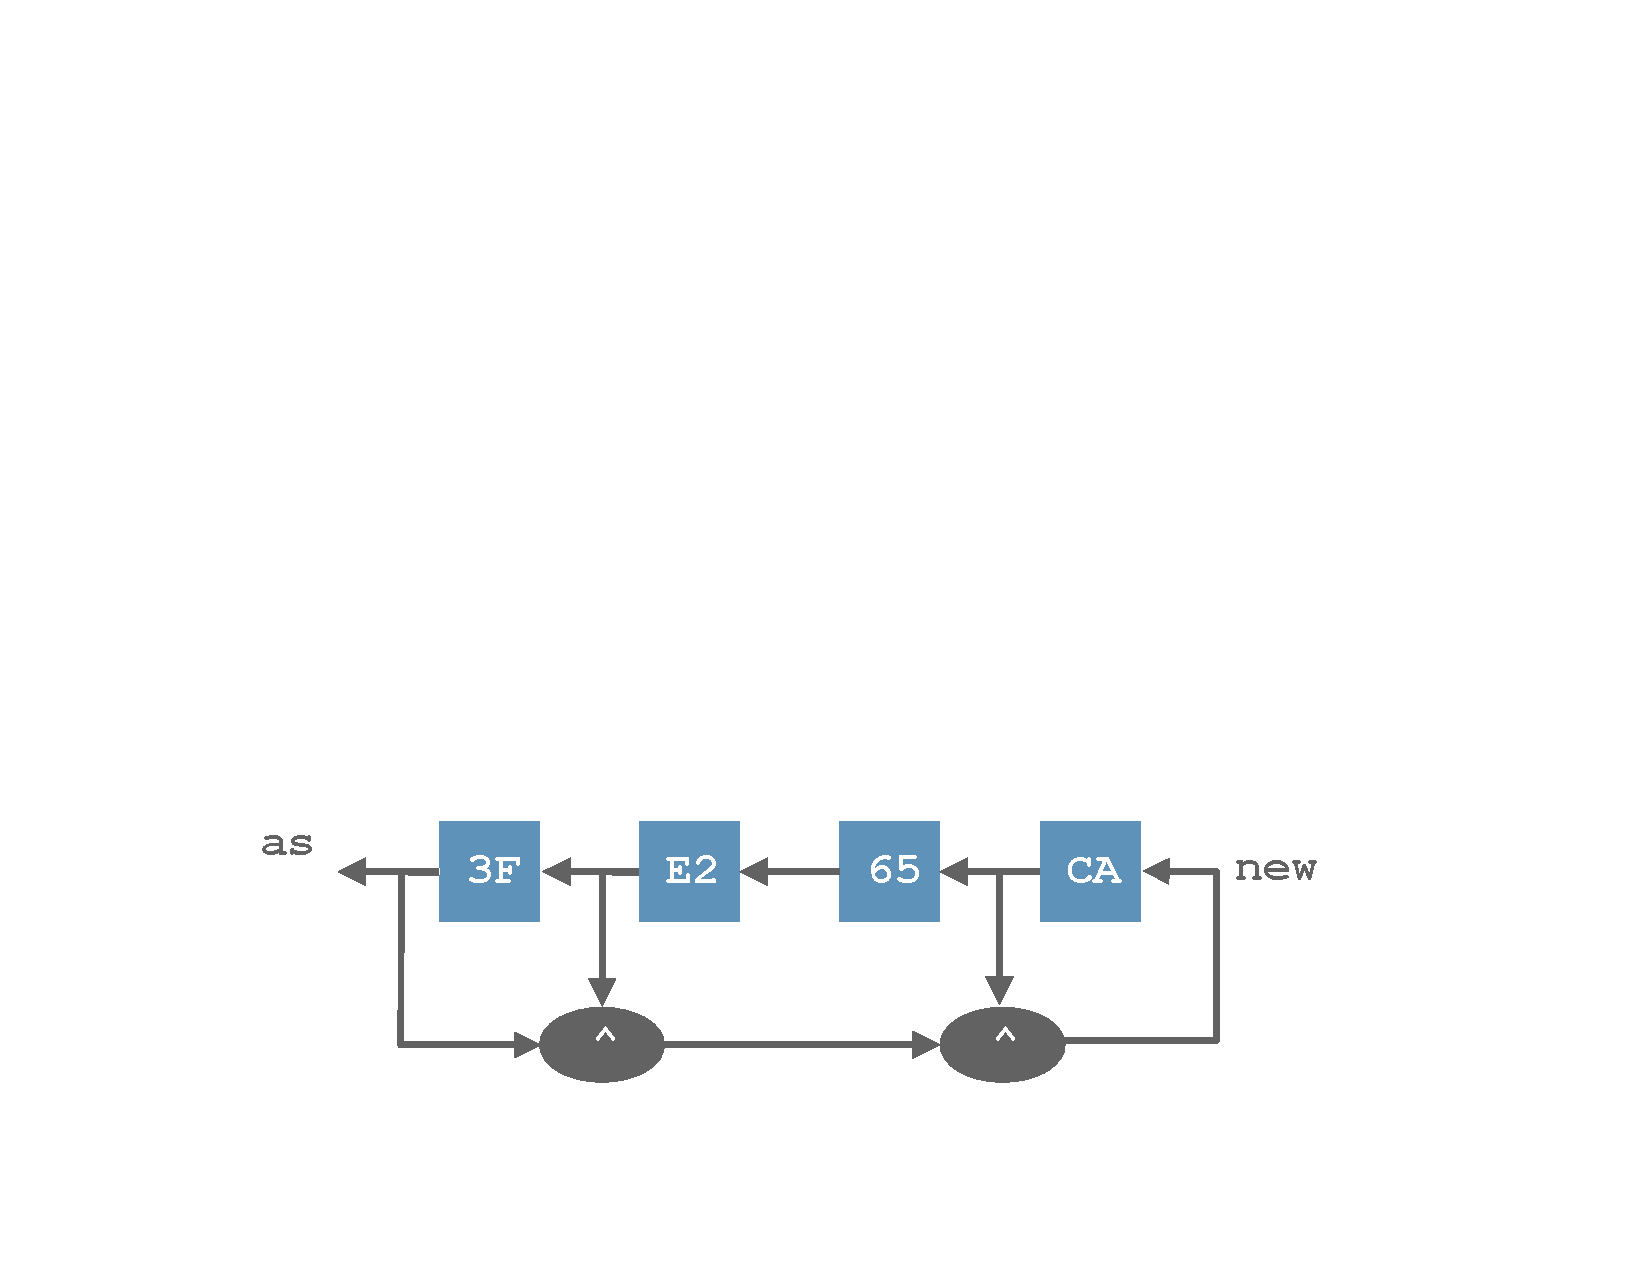
\includegraphics[width=3.5in]{crashCourse/streamDiagram.pdf}
\caption{Equation for producing a stream of {\tt as}}
\label{fig:streamDiagram}
\end{figure}

In this diagram the stream is seeded with four initial values ({\tt
  3F, E2, 65, CA}). The subsequent elements ({\tt new}) are appended
to the stream, and are computed by xor-ing the current stream element
with two additional elements extracted from further into the stream.
The output from the stream is a sequence of values, known as 'a's.

The Cryptol code corresponding to this stream equation is:
\begin{code}
  as  = [0x3F, 0xE2, 0x65, 0xCA] # new
    where
      new = [ a ^ b ^ c | a <- as
                        | b <- drop`{1} as
                        | c <- drop`{3} as ]
\end{code}

% \vfill
% \eject 
\todo[inline]{Make sure pagination looks good, particularly for figures.}

\begin{Exercise}\label{ex:streamEq}
  Write the Cryptol code corresponding to the stream equation in
  Figure~\ref{fig:streamExercise}:
\end{Exercise}
\begin{figure}[htbp]
\centering
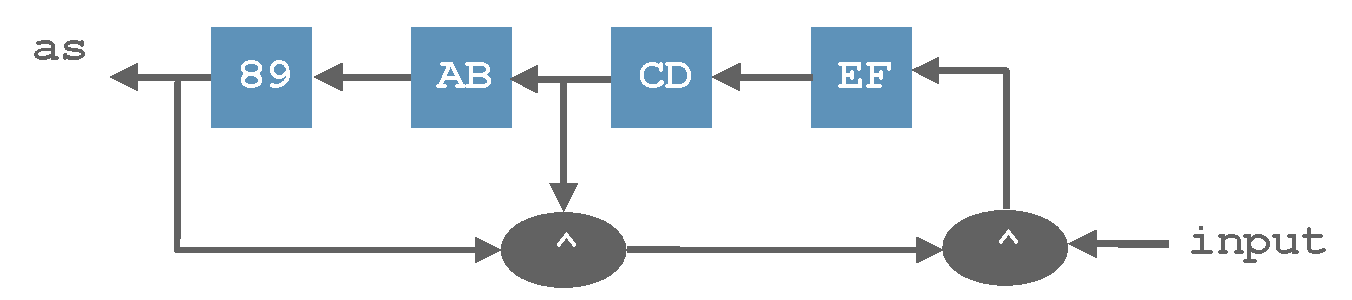
\includegraphics[width=4in]{crashCourse/streamExercise}
\caption{Equation for producing a stream of {\tt as} from an initial
  seed and an input stream.}
\label{fig:streamExercise}
\end{figure}

\todo[inline]{Update diagram so that the output is called \texttt{xs}
  to match the solution and we avoid getting an error from Cryptol
  about redeclaration of \texttt{as}.}

\begin{Answer}\ansref{ex:streamEq}
\begin{code}
  xs input = [0x89, 0xAB, 0xCD, 0xEF] # new
     where new = [ a ^ b ^ c | a <- as
                             | b <- drop`{2} as
                             | c <- input ]
\end{code}
\end{Answer}

%=====================================================================
\section{Type synonyms}
\label{sec:tsyn}
\sectionWithAnswers{Type synonyms}{sec:tsyn}\indTypSynonym

\todo[inline]{Motivate type synonyms better; NQueens with nice
  synonyms is a good example.}

\todo[inline]{Should we insert a section on currying-style functions
  vs. tuples here?}

Types in Cryptol can become fairly complicated, especially in the
presence of records.  Even for simple types, meaningful names should
be used for readability and documentation.  Type synonyms allow users
to give names to arbitrary types.  In this sense, they are akin to
{\tt typedef} declarations in C~\cite{TheCProgrammingLanguage}.
However, Cryptol's type synonyms are significantly more powerful than
C's {\tt typedef}'s, since they can be parameterized by other types,
much like in Haskell~\cite{Has98}.

\todo[inline]{Add a discussion of N-queens or AES or something more compelling
  to show off type synonyms.}

Here are some simple type synonym definitions:
\begin{code}
  type Word8       = [8]
  type CheckedWord = (Word8, Bit)
  type Point a     = {x : [a], y : [a]}
\end{code}

\todo[inline]{2.0: Rewrite this paragraph and much of this section.}

Type synonyms are either unparameterized (as in {\tt Word8} and {\tt
  CheckedWord}, or parameterized with other types (as in {\tt Point}).
Synonyms may depend upon other synonyms, as in the {\tt CheckedWord}
example.  Once the synonym is given, it acts as an additional name for
the underlying type, making it much easier to read and
maintain.  

For instance, we can write the function that returns the x-coordinate
of a point as follows:
\begin{code}
  xCoord : {a} Point a -> [a]
  xCoord p = p.x
\end{code}

Note that type synonyms, while maintained within the type and value
context shown via the \texttt{:browse} command, are
\emph{value-based}, not \emph{name-based}.  When viewed from the
types-as-sets interpretation, two types in Cryptol are synonymous if
their values happen to be equal.  

For example, consider the following declarations:
\begin{code}
  type Word8     = [8]
  type Word8'    = [8]
  type B         = Word8
  type A         = B
  type WordPair  = (Word8, Word8')
  type WordPair' = (Word8', Word8)

  foo: Word8 -> Bit
  foo x = True

  bar: Word8' -> Bit
  bar x = foo x
\end{code}
Within this type context, while six \emph{names} are declared, only
\emph{two} types are declared (\texttt{[8]} and the pair \texttt{([8],
[8])}.  Likewise, the function types of \texttt{foo} and \texttt{bar}
are identical, thus \texttt{bar} can call \texttt{foo}.

\begin{Exercise}\label{ex:tsyn:1}
  Define a type synonym for 3-dimensional points and write a function
  to determine if the point lies on any of the 3 axes.
\end{Exercise}
\begin{Answer}\ansref{ex:tsyn:1}
  A point is on the $a^{\text{th}}$ axis if its non-$a^{\text{th}}$
  components are $0$. Hence we have:
\begin{code}
  type Point3D a = {x : [a], y : [a], z : [a]}

  onAnAxis : {a} (fin a) => Point3D a -> Bit
  onAnAxis p = onX || onY || onZ
    where onX = (p.y == 0) && (p.z == 0)
          onY = (p.x == 0) && (p.z == 0)
          onZ = (p.x == 0) && (p.y == 0)
\end{code}
\todo[inline]{Reflect upon this example.}
\end{Answer}

\paragraph*{Predefined type synonyms} The following type synonyms are
predefined in Cryptol:
\begin{Verbatim}
  type Bool = Bit
  type Char = [8]
  type String n = [n]Char
  type Word n = [n]
\end{Verbatim}
For instance, a {\tt String n} is simply a sequence of precisely n
8-bit words.\indTSWord\indTSString\indTSBool

\todo[inline]{Discussion of \texttt{String} as a type synonym is an
  important example, so more discussion is warranted.}

%=====================================================================
\section{Type classes}\indTypeClasses
\label{sec:type-classes}

\todo[inline]{This section needs a full rewrite.}

\todo[inline]{Add discussion of Haskell's type classes and other
  typeclass-like things.}

Type classes are a way of describing behaviors shared by multiple
types.  As an example, consider the type of the function {\tt ==}:
\begin{Verbatim}
    Cryptol> :t (==)
    == : {a} (Cmp a) => a -> a -> Bit
\end{Verbatim}

This operator type is interpreted ``equality is an operator that takes
two objects of any single type that can be compared and returns a
Bit.''  

Cryptol defines exactly two basic type classes: {\tt Cmp} and {\tt
  Arith}.  These appear in the type signature of operators and
functions that require them.  If a function you define calls, for
example, {\tt +}, on two arguments both of type {\tt a}, the type
constraints for {\tt a} will include {\tt (Arith a)}.

The \texttt{Cmp} typeclass includes the binary relation operators
\texttt{<}, \texttt{>}, \texttt{<=}, \texttt{>=}, \texttt{==}, and
\texttt{!=}, as well as the binary functions \texttt{min} and
\texttt{max}.  Note that equality is defined on function types (i.e.,
\texttt{{a b} (Cmp b) => (a -> b) -> (a -> b) -> a -> Bit}).  Unlike
in many other languages, equality and comparison are bundled into a
single typeclass.

The \texttt{Arith} typeclass include the binary operators \texttt{+},
\texttt{-}, \texttt{*}, \texttt{/}, \verb+%+, \verb+^^+, as well
as the unary operators \texttt{lg2} and \texttt{-}.

\begin{Exercise}\label{ex:tvar:1}
  Without including an explicit type declaration, define a function
  that Cryptol infers has the following type:
\begin{Verbatim}
  cmpArith : {a,b} (Cmp a, Arith b) => a -> a -> b -> b
\end{Verbatim}
\end{Exercise}
\begin{Answer}\ansref{ex:tvar:1}
This code:
\begin{code}
  cmpArith x y z = if x == y then z else z+z
\end{code}
yields the inferred type:
\begin{Verbatim}
  cmpArith : {a, b} (Arith b, Cmp a) => a -> a -> b -> b
\end{Verbatim}
\end{Answer}

%=====================================================================
\section{Type vs. value variables}\indTypeVariables
\label{sec:type-vs.-value}

\todo[inline]{Rewrite this whole section to better clarify object- vs. type
  variables, their scope and limitations, where they can be left
  abstract and when and where they must be concretized, etc.}

Its powerful type system is one of the key features of Cryptol.  We
have encountered many aspects of types already.  You may have noticed,
in functions such as {\tt groupBy}, that when you call a function in
Cryptol, there are two kinds of parameters you can pass: {\it value
  variables} and {\it type variables}.

Consider the \emph{groupBy} function that we previously examined in
\autoref{ex:poly:groupBy}.  Recall that \texttt{groupBy}'s type is:
\begin{verbatim}
    groupBy : {each, parts, elem} (fin each) =>
              [parts * each]elem -> [parts][each]elem
\end{verbatim}
When applying \texttt{groupBy}, one typically specifies a concrete
value for the formal parameter \texttt{parts}:
\begin{Verbatim}
    Cryptol> groupBy`{parts=3}[1..12]
    [[1, 2, 3, 4], [5, 6, 7, 8], [9, 10, 11, 12]]
\end{Verbatim}
In this example, the term {\tt\Verb|`{parts=3}|} passes 3 to the {\tt
  parts} type variable argument, and the {\tt [1..12]} is passing a
sequence as the first (and only) {\it value argument}, \texttt{elem}.

A \emph{value variable} is the kind of variable you are used to from
normal programming languages.  These kinds of variable represent a
normal run-time value.  

A \emph{type variable}, on the other hand, allows you to express
interesting (arithmetic) constraints on \emph{types}. These variables
express things like lengths of sequences or relationships between
lengths of sequences.  Type variable values are computed
statically---they never change at runtime\footnote{In this way,
  they are similar (but more expressive than) templates in languages
  like C++ or Java. If you want to learn more about this area, look up
  the term ``type-level naturals''.}.

%~~~~~~~~~~~~~~~~~~~~~~~~~~~~~~~~~~~~~~~~~~~~~~~~~~~~~~~~~~~~~~~~~~~~~
\subsection{Positional vs. named type
  arguments}\indTypePositionalArguments
\label{sec:positional-vs.-named}

Cryptol permits type variables to be passed either by name (as in {\tt
  \Verb|`{parts=3}|} above), or by position (leaving out the name).
For functions you define, the position is the order in which the type
variables are declared in your function's type signature. If you are
not sure what that is, you can always use the {\tt :t} command to find
out the position of type variables. 

For example:
\begin{Verbatim}
    Cryptol> :t groupBy
    groupBy : {each, parts, elem} 
              (fin each) => [parts * each]elem 
                         -> [parts][each]elem
\end{Verbatim}
tells us that that {\tt parts} is in the second position of {\tt
  groupBy}'s type signature, so the positional-style call equivalent
to our example is:
\begin{Verbatim}
    Cryptol> groupBy`{_,3}[1..12]
\end{Verbatim}

Note the use of an underscore in order to pass \texttt{3} in the
second position.  Positional arguments are most often used when the
type argument is the first argument and when the name of the argument
does not add clarity.  The {\tt groupBy\Verb|`{_,3}|} is not as self-
explanatory as {\tt groupBy\Verb|`{parts=3}|}.  On the other hand, our
use of positional arguments to {\tt take} in previous chapters is very
clear, as in:
\begin{Verbatim}
    Cryptol> take`{3}[1..12]
    [1, 2, 3]
\end{Verbatim}

\begin{tip}
  Cryptol programs that use named arguments are more maintainable and
  robust during program evolution.  E.g., you can reorder paramters or
  refactor function definitions much more easily if invocations of
  those functions use named, rather than positional, arguments.
\end{tip}

\todo[inline]{What are the implications to type inference, especially
  resolution, in the presence of positional arguments.}

%~~~~~~~~~~~~~~~~~~~~~~~~~~~~~~~~~~~~~~~~~~~~~~~~~~~~~~~~~~~~~~~~~~~~~
\subsection{Type context vs. variable context}\indTypeContext
\label{sec:type-context-vs}

You have seen, in the discussion of type variables above, that Cryptol
has two kinds of variables -- type variables and value variables. Type
variables normally show up in type signatures, and value variables
normally show up in function definitions. Sometimes you may want to
use a type variable in a context where value variables would normally
be used.  To do this, use the backtick character {\tt \Verb|`|}.  

The definition of the built-in {\tt width} function is a good example
of the use of backtick:
\begin{Verbatim}
    width : {bits,len,elem} (fin len, fin bits, bits >= width len) =>
            [len] elem -> [bits]
    width _ = `len
\end{Verbatim}

\begin{tip}
  Note there are some subtle things going on in the above definition
  of \texttt{width}.  First, arithmetic constraints on types are
  position-independent; properties of formal parameters early in a
  signature can depend upon those late in a signature.  Second, type
  constraints can refer to not only other functions, but recursively
  to the function that is being defined (either directly, or
  transitively).

  Type constraints can get pretty crazy in practice, especially deep
  in the signature of crypto code subsystems.  Our suggestion is that
  you should not chase the dragon's tail of feedback from the
  typechecker in attempting to massage your specification's types for
  verification.  Instead, think carefully about the meaning and
  purpose of the concepts in your specification, introduce appropriate
  type synonyms, and ensure that the specification is clear and
  precise.  Trust that the interpreter and the verifier will do the
  right thing.
\end{tip}

The bounds in a finite sequence literal (such as {\tt [1 .. 10]}) in
Cryptol are type-level values because the length of a sequence is part
of its type.  Only type-level values can appear in a finite sequence
definition.  You cannot write {\t [a .. b]} where either {\tt a} or
{\tt b} are arguments to a function.  On the other hand, an infinite
sequence's type is fixed ({\tt [inf]a}), so the initial value in an
infinite sequence can be a runtime variable or a type variable, but
type variables are escaped here using a {\tt \Verb|`|}.

\todo[inline]{Add an example of this here.  Rewrite if something great
  occurs to us.}

\todo[inline]{A proper discussion of type-context vs.~value-context is
  necessary here, and it should be formalized as part of the type
  system and type-inference algorithm, of course.}

This is probably obvious, but there is no way to get a value variable
to appear in a type context.  Types must be known at ``compile time,''
and (non-literal) values are not, so there is no way to use them in
that way.

\todo[inline]{It is more subtle than this because we do not have a proper
  semantic for when arithmetic terms in types (or expressions, for
  that matter!) are evaluated.}

%~~~~~~~~~~~~~~~~~~~~~~~~~~~~~~~~~~~~~~~~~~~~~~~~~~~~~~~~~~~~~~~~~~~~~
\subsection{Inline argument type declarations}\indTypeInline
\label{sec:inline-argument-type}

So far when we have defined a function, we have declared the type of
its arguments and its return value in a separate type declaration.
When you are initially writing code, you might not know exactly what a
function's full type is (including the constraints), but you may know
(and need to express) the types of the function's arguments. Cryptol's
syntax for this should look familiar:
\begin{code}
  addBytes (x:[8]) (y:[8]) = x + y
\end{code}

This defines a function that takes two bytes as input, and returns their sum.
Note that the use of {\tt( )}'s is mandatory.

Here is a more interesting example:
\begin{code}
  myWidth (x:[w]a) = `w
\end{code}

\todo[inline]{Why is this more interesting?  What are the reflections the
  reader should have?}

%=====================================================================
\section{The road ahead}
\label{sec:road-ahead}

In this introductory chapter, we have seen essentially all of the
language elements in Cryptol. The concepts go deeper, of course, but
you now have enough knowledge to tackle large Cryptol programming
tasks. As with any new language, the more exercises you do, the more
you will feel comfortable with the concepts. In fact, we will take
that point of view in the remainder of this document to walk you
through a number of different examples (both small and large),
employing the concepts we have seen thus far.

%%% Local Variables: 
%%% mode: latex
%%% TeX-master: "../main/Cryptol.tex"
%%% End: 
